\documentclass[11pt]{article}
\usepackage[T1]{fontenc}
\usepackage{lmodern}
\usepackage[margin=1in]{geometry}
\usepackage{amsmath,amssymb,amsthm,mathtools}
\usepackage{microtype}
\usepackage{enumitem}
\usepackage{tikz}
\usetikzlibrary{arrows.meta}
\usepackage[numbers,sort&compress]{natbib}
\usepackage[colorlinks=true,linkcolor=blue!45!black,citecolor=blue!45!black,urlcolor=blue!45!black]{hyperref}
\usepackage[nameinlink,capitalise,noabbrev]{cleveref}
\hypersetup{
 pdftitle={An Endpoint Gradient Bound for the Centered Disk Maximal Operator},
 pdfauthor={OpenAI},
 pdfsubject={Planar endpoint Sobolev regularity of the centered disk maximal operator}
}
\newcommand{\R}{\mathbb R}
\newcommand{\N}{\mathbb N}
\newcommand{\dd}{\mathop{}\!\mathrm{d}}
\newcommand{\1}{\mathbf 1}
\newcommand{\E}{\mathbb E}
\newcommand{\Prob}{\mathbb P}
\newcommand{\abs}[1]{\left|#1\right|}
\newcommand{\norm}[1]{\left\|#1\right\|}
\DeclareMathOperator{\Lip}{Lip}
\DeclareMathOperator{\supp}{supp}
\DeclareMathOperator{\dist}{dist}
\DeclareMathOperator{\Var}{Var}
\newtheorem{theorem}{Theorem}[section]
\newtheorem{lemma}[theorem]{Lemma}
\newtheorem{proposition}[theorem]{Proposition}
\newtheorem{corollary}[theorem]{Corollary}
\theoremstyle{definition}
\newtheorem{definition}[theorem]{Definition}
\theoremstyle{remark}
\newtheorem{remark}[theorem]{Remark}
\numberwithin{equation}{section}
\setlist[enumerate]{label=(\roman*),leftmargin=2em}
\setlength{\emergencystretch}{1.5em}
\title{An Endpoint Gradient Bound for the Centered Disk Maximal Operator}
\author{OpenAI}
\date{September 26, 2026}
\begin{document}
\maketitle
\begin{abstract}
We prove the endpoint gradient bound $\|\nabla Mf\|_1\le C\|\nabla f\|_1$
for every real-valued $f\in W^{1,1}(\R^2)$, where $Mf(x)$ is the supremum
of the averages of $|f|$ over disks centered at $x$, and $C$ is an absolute
constant. The maximal function belongs to $W^{1,1}_{\mathrm{loc}}(\R^2)$
and has a globally integrable weak gradient. This gives a positive resolution
of the planar centered-disk case of the endpoint question of Haj{\l}asz and
Onninen.
\end{abstract}
\section{Introduction}\label{sec:introduction}

For $f\in L^1_{\mathrm{loc}}(\R^2)$, the centered disk maximal function is
\[
 Mf(x)=\sup_{r>0}\frac1{\pi r^2}\int_{B(x,r)}|f(y)|\,\dd y,
 \qquad B(x,r)=\{y\in\R^2:|y-x|<r\}.
\]
Every averaging disk is centered at the point of evaluation, and all
positive radii are allowed. Kinnunen proved that this operator is
bounded on $W^{1,p}$ for $1<p<\infty$
\cite[Theorem~1.4]{Kinnunen1997}. The pointwise control of its gradient
by $M(|\nabla f|)$ gives the corresponding norm bound through the
strong $L^p$ maximal inequality. At $p=1$ that last step fails.
Haj{\l}asz and Onninen asked whether the gradient estimate itself
nevertheless survives \cite[Question~1]{HajlaszOnninen2004}.
We give a positive resolution of the planar centered-disk case of
their endpoint question.

\begin{theorem}\label{thm:main}
There is an absolute constant $C<\infty$ such that, for every
real-valued $f\in W^{1,1}(\R^2)$, the function $Mf$ is locally
integrable, belongs to $W^{1,1}_{\mathrm{loc}}(\R^2)$, and satisfies
\begin{equation}\label{eq:main}
 \int_{\R^2}|\nabla Mf|\,\dd x
 \le C\int_{\R^2}|\nabla f|\,\dd x.
\end{equation}
In particular, its distributional derivatives are represented by
globally integrable functions.
\end{theorem}

Here $W^{1,1}(\R^2)$ is the inhomogeneous Sobolev space: the input and
its weak first derivatives are globally integrable. Vector norms are
Euclidean. No radiality or compact-support condition is imposed on
the input. The maximal function itself need not be globally
integrable, even for a nonzero nonnegative smooth function of compact
support. The constant in \eqref{eq:main} is finite and absolute; its
optimal value is not determined. The argument below concerns disks
in the plane.

\subsection{The signed estimate behind the theorem}

The intermediate estimate retains the sign of the input. For real
$g\in C_c^\infty(\R^2)$, put
\[
 A_tg(x)=\frac1{\pi t^2}\int_{B(x,t)}g(y)\,\dd y,
 \qquad S_{a,b}g(x)=\sup_{a\le t\le b}A_tg(x).
\]
For fixed $0<a\le b<\infty$, this envelope is compactly supported and
Lipschitz. The issue is to bound its gradient uniformly as the range
of radii grows.

\begin{proposition}[Signed finite-band estimate]\label{prop:finite-band}
There is an absolute constant $C$ such that, for every real
$g\in C_c^\infty(\R^2)$ and $0<a\le b$ with $b/a$ a power of two, including one,
\begin{equation}\label{eq:intro-band}
 \int_{\R^2}|\nabla S_{a,b}g|\,\dd x
 \le C\int_{\R^2}|\nabla g|\,\dd x.
\end{equation}
The constant is independent of $a$, $b$, and the number of dyadic
radius scales between them.
\end{proposition}

The proof of Proposition~\ref{prop:finite-band} is given in Section~\ref{sec:assembly}, after the local and multiscale estimates described below. A single radius, $a=b$, is covered directly by convolution. The signed form of Proposition~\ref{prop:finite-band} has a specific purpose in the final regularity argument.
After extension to Sobolev inputs, one applies it to
$g_Q=\chi_Q(g-c_Q)$, where $c_Q$ is a local mean and $\chi_Q$ equals
one on the small disks being tested. On those disks,
$A_tg_Q=A_tg-c_Q$, so the corresponding envelopes have the same
gradient. Poincar\'e's inequality then bounds $\|\nabla g_Q\|_1$
by the gradient of $g$ on a slightly larger square. The function
$g_Q$ can take both signs. Signed averages also occur in Weigt's
dyadic and uncentered cube estimates
\cite{Weigt2023Dyadic,Weigt2025Cubes}; their role here is to permit
this local subtraction.

\subsection{Earlier endpoint results}

In one dimension, Tanaka proved an $L^1$ derivative bound for the
uncentered maximal operator \cite[Theorem~1]{Tanaka2002}.
Aldaz and P\'erez L\'azaro extended the result to inputs of bounded
variation, established absolute continuity of the maximal function,
and obtained the sharp variation constant $1$
\cite[Theorem~2.5]{AldazPerezLazaro2007}.
Kurka proved a variation bound with an absolute constant for the
centered operator on functions of bounded variation, together with
local Sobolev regularity and an integrable derivative for Sobolev
inputs \cite[Theorem~1.2 and Corollary~1.4]{Kurka2015}.
The ordering of intervals used in these arguments does not directly
organize a family of centered disks.

In higher dimensions, Aldaz and P\'erez L\'azaro proved regularity for
block-decreasing inputs, invariant under coordinate sign changes and
nonincreasing in each positive coordinate, and uncentered maximal operators over balls of
unconditional norms; their weak-gradient conclusion applies, in particular,
to block-decreasing $W^{1,1}$ input and Euclidean balls
\cite[Theorem~11]{AldazPerezLazaro2009Block}.
Luiro proved the $L^1$ gradient estimate for
radial Sobolev input and the uncentered ball operator
\cite[Theorem~3.12]{Luiro2018Radial}.
Weigt established variation bounds for the dyadic maximal operator
\cite{Weigt2023Dyadic} and for the uncentered maximal operator over
axis-parallel cubes \cite[Theorem~1.1]{Weigt2025Cubes}.
Their geometry and indexing differ from centered disks. Moreover,
a variation estimate controls a derivative measure, which may still
have a singular part. For fractional orders $0<\beta<1$, Beltran and Madrid established
centered endpoint gradient bounds for radial $W^{1,1}$ input
\cite[Theorem~1.2]{BeltranMadrid2020CenteredFractional}.
Weigt subsequently proved endpoint gradient estimates for both
the centered and uncentered operators
\cite[Theorem~1.1]{Weigt2022Fractional}. The positive order restricts
overlap among optimizing balls in that proof; the mechanism
degenerates at order zero.

Lahti and Weigt's conditional regularity theorem upgrades local
bounded variation of the centered maximal function to local Sobolev
regularity when the input is Sobolev
\cite[Theorem~1.2]{LahtiWeigt2025}. It assumes the requisite variation
bound. We prove that bound and then remove the singular part directly
using the signed localization above. Finally, boundedness and
continuity of the gradient map are distinct questions. The
one-dimensional continuity results of Carneiro, Madrid and Pierce
for the uncentered operator \cite{CarneiroMadridPierce2017}, and of
Gonz\'alez-Riquelme for the centered operator
\cite{GonzalezRiquelme2023Continuity}, concern this further issue.
Theorem~\ref{thm:main} asserts the planar norm estimate.

\subsection{How the finite-band estimate is proved}

Write
\begin{equation}\label{eq:signed-average}
 u_t=A_tg,\qquad h=(\nabla g)\,\dd x,\qquad
 V=|h|(\R^2)=\int|\nabla g|.
\end{equation} Scaling reduces
Proposition~\ref{prop:finite-band} to radii in $[2^{-m},1]$.
The proof has one geometric input and two separate multiscale
constructions. The first construction organizes scalar cancellation;
the second chooses directions and pays for their changes in both
scale and space.

\paragraph{Disk moments and concentration in a shell.}
At an interior maximizing radius, the radial derivative of $u_t$
vanishes. A rotational moment vanishes on every disk. In complex
notation these identities give a zero first moment, which is
preserved by suitable positive mixtures of nearby disks. Variations
of optimizing balls also produce weighted-gradient identities in
Luiro's work \cite[Lemmas~2.2 and~2.4]{Luiro2018Radial}; we derive
the identities needed for centered signed averages directly.

Identify $\R^2$ with $\mathbb C$, let $x$ be the disk center, and let
$z$ be a point of its thin boundary shell. The purpose of the moment
identity is visible in the affine factor
\[
 W_z(y)=1-\frac{\overline{y-x}}{\overline{z-x}}.
\]
This factor vanishes at $z$. Inserting it in a difference of balanced
disk kernels therefore makes mass near $z$ inexpensive. This leads
to the geometric question: when is almost all relevant shell mass
concentrated near one point? A sweep by nested disks tangent at that
point answers it outside one exceptional set of centers, uniformly
over every radius in the band. Crucially, it requires a bound on
positive mass only in an inner disk; the error mass is controlled
separately.

These observations yield a local directional estimate. On a square
of side $r$, decompose $h$ into positive measures with directions
in one cone and localized errors. Errors smaller than the
observation scale have zero total vector mass; errors at scale
$r$ are charged their full variation. An
error of variation $b$ supported at scale $s\le r$ is charged
$b(s/r)^\alpha$, with a fixed $\alpha=1/100$. The resulting sum
controls the integral over the square of the supremum, over locally
maximizing radii, of the gradient component pointing against the
cone. Companion estimates handle band endpoints and the value
oscillation
\[
 v_k(x)=\sup_{0<t,t'\le4r_k}|u_t(x)-u_{t'}(x)|,
 \qquad r_k=2^{-k}.
\]
Those estimates include the endpoint arguments and the comparison
of successively narrower kernels; shell concentration alone does
not supply them.

\paragraph{Scalar cancellation and a common price for each cell.}
Let $\phi_q$ be the product of the two one-dimensional tents at a
vertex $q$ of the level-$k$ dyadic grid: each factor equals one at its
vertex coordinate and decreases linearly to zero one mesh width away. Set $h_q=\int\phi_q\,\dd h$, $a_q=|h_q|$.
The tents form positive partitions of unity and refine positively
onto finer grids. We express vectors in each of finitely many bases formed by the two
boundary directions of a cone. For each scalar coordinate, we start
with the actual signed density at the finest level.
Pair its positive and negative parts in equal masses, retain the
constant-sign remainder, and repeat this operation on the weighted
remainders at each parent. This bottom-up construction retains
the support and birth level of every pair, including cancellation
inside the finest tents. Its identity is an identity of measures,
so there is no unrepresented terminal density.

The masses paired at successive levels form a telescoping sum.
Charging each pair at coarser
observation scales with the factor $(s/r)^\alpha$ gives a
nonnegative price $D_Q$ for every dyadic cell, with
\begin{equation}\label{eq:overview-price-budget}
 \sum_Q D_Q\le CV.
\end{equation}
One price works for every direction in the fixed finite palette.
The local estimates then cost $D_Q$ together with appropriate
nearby vector masses $a_q$ at the observation scale. Multiscale oscillation budgets already
play a role in Kurka's one-dimensional proof
\cite[Lemma~1.5]{Kurka2015}; the scalar measure decomposition and
its common prices are proved here.

\paragraph{Vector particles and the cost of choosing directions.}
The remaining vector masses require a different construction.
Vector refinement makes their total increase with the level,
while keeping it at most $V$. We realize these masses by a finite
positive measure on refinement paths, adding mass when needed
and recording its birth level. This construction preserves the
complete path, including levels before birth, so that it can
compare choices of direction made from the first scale onward.
These vector particles differ from the scalar cancelling pairs:
their role is to turn estimates along paths into sums of vector-mass
charges over cells.

Two costs must be controlled. A change of direction starts a new
run of radius scales and creates endpoint terms. Spatial variation
of the choice of direction creates derivatives of its weights
when we integrate by parts. Section~\ref{sec:labels} constructs a finite-state
law at each point $x$ and bounds sums of both costs, weighted
by these vector masses, by $CV$, with the spatial suprema needed
for the cell estimates. Vector-additivity
defects control changes along particles, and comparison at nearby
points transfers that control to the spatially varying law.

\paragraph{Assembly and cancellation of differentiated rows.}
After the common prices and the direction costs have been
bounded, we assemble the radius bands. A run is a maximal consecutive
interval of scales carrying the same direction. For each history,
apply the local directional estimate to the supremum over the
radii of every run, then average over histories. The common
prices and the bounds for direction changes pay for the
unfavorable components and the endpoints of runs.

For each run, subtract the average at its starting scale from
its envelope; the endpoint estimates pay for the gradients of
these baselines. The vector quantity to be integrated by parts
is the sum of the resulting envelopes multiplied by their run
directions. Its history weight depends on $x$. If
$\pi_k(x;n,n')$ is the probability of passing from direction $n$
to direction $n'$ at step $k$, normalization of each row gives
\[
 \sum_{n'}\nabla_x\pi_k(x;n,n')=0.
\]
Before taking absolute values, we can therefore subtract the
analogous vector sum for the preceding history, ending its last
run at level $k-1$. That sum is independent of the next direction.
The difference contains only extensions of the last run and new
runs, and is bounded by $C\sum_{l\ge k}v_l$. The local value
estimate contributes the scale $r_l$, while a differentiated
transition row has scale $1/r_k$. Their ratio $r_l/r_k$ is
exactly the geometric weight controlled by the direction-cost
estimate. Together with the common-price budget, these bounds
give \eqref{eq:intro-band}.

\subsection{From the finite-band estimate to a weak gradient}

Approximation extends Proposition~\ref{prop:finite-band} to signed Sobolev
inputs. Applying it to $g=|f|$ and increasing the radius bands first
gives a finite vector Radon measure representing the derivative
of $Mf$. To prove that this measure has no singular part, fix a
compact null set and a positive radius threshold. The envelope
over larger radii is Lipschitz, so its contribution vanishes
as the neighborhood of the null set shrinks. For small radii, the signed
cutoff and local mean subtraction described above reduce the cost
to the integral of $|\nabla g|$ within a fixed multiple of the
threshold distance. After shrinking the neighborhood, let the
radius threshold tend to zero. This gradient integral then
vanishes as well. Inner regularity gives absolute continuity
of the derivative measure and proves Theorem~\ref{thm:main}.

Lower-radius Lipschitz truncations appear in Haj{\l}asz and
Mal\'y \cite[Lemma~8]{HajlaszMaly2010}, and local/nonlocal
splitting with subtraction of an input mean appears in Saari
\cite[Section~3.1]{Saari2019}. The signed estimate above supplies
the gradient-only localization used here.

Section~\ref{sec:local} proves disk cancellation and the local estimates.
Section~\ref{sec:prices} gives scalar refinement and common prices; Section~\ref{sec:labels}
constructs the vector particles and spatial label law.
Section~\ref{sec:assembly} assembles the finite bands, and Section~\ref{sec:extension} passes to
Sobolev input and removes the singular part. An analytic appendix records the Sobolev
calculus, square localization, and vector-measure facts in the
forms used in the final step. \subsection{Conventions}


A constant denoted by $C$ may increase between occurrences.
All parameters, including cone apertures, finite direction nets and
geometric neighborhood sizes, are fixed absolute choices. In a local
lemma the explicitly listed cone and support constants are allowed
dependencies. No constant depends on the number of radius scales.

For a vector measure $\nu$, $|\nu|$ denotes its total variation.
For a real number $a$, $a_+=\max(a,0)$.
A supremum of nonnegative quantities over an empty set is zero.
When $\nabla u_t$ is written, the radius is held fixed.
We use the classical strong $L^p$ maximal inequality for $p>1$
\cite[(1.2)]{Kinnunen1997}; a general account is given in
\cite[Chapter~I]{Stein1970}. The analytic appendix records the
remaining standard inputs in the forms used here.

\section{Cancellation at disks and three local bounds}
\label{sec:local}

Throughout this section, $g\in C^\infty(\R^2)$ is real valued,
$h=\nabla g\,dx$, and $u_t=A_tg$. The averages are signed. No
compact-support assumption on $g$ is needed for the local estimates.
Our goal is to control three quantities on a unit square: unfavorable
directional gradients at locally maximizing radii, gradients at band
maxima and endpoints, and differences of averages. The common input is
a decomposition of the gradient into positive directions and error
pieces, with small support and zero total mass below size one. The discount on the latter errors will make the
scale sum in Section~\ref{sec:prices} finite.
We fix
\begin{equation}\label{eq:local-alpha}
\alpha=\frac1{100}.
\end{equation}
An equality of measures on an open set means equality of their
restrictions there. The component measures themselves will always
remain defined on the whole plane.

\begin{lemma}[Local estimates]\label{lem:local}
Let $Q$ be a square of side length one and let
$\Omega=\{y:\dist(y,Q)<10\}$. Suppose that, on $\Omega$,
\begin{equation}\label{eq:local-decomposition}
h=\sum_i v_i\sigma_i+\beta,
\qquad \beta=\sum_d\beta_d.
\end{equation}
The sums are finite. The measures in the sums are finite, defined on
$\R^2$, and absolutely continuous with respect to Lebesgue measure.
Each $\sigma_i$ is nonnegative and each $v_i$ is a constant unit vector.
For each $d$, write $m_d=|\beta_d|(\R^2)$ and assign a number
$s_d\in(0,1]$. If $s_d<1$, assume that
$\beta_d(\R^2)=0$ and that $\beta_d$ is supported in a ball of radius
at most $C_s s_d$, where $C_s$ is fixed. Set
\[
S=\sum_i\sigma_i,
\qquad A=\sum_d s_d^\alpha m_d.
\]
For $x\in Q$, define
\begin{align*}
\mathcal I(x)
&=\{r\in[1,2]:u_r(x)\ge u_t(x)
                 \text{ for every }t>0\text{ with }|t-r|\le1/4\},\\
\mathcal J(x)
&=\{r\in[1,2]:u_r(x)=\max_{1\le t\le2}u_t(x)\}\cup\{1,2\}.
\end{align*}
Then the following estimates hold.
\begin{enumerate}
\item \emph{Unfavorable directional gradients.} If $e$ is a unit vector and $e\cdot v_i\ge\kappa>0$ for all $i$,
then
\begin{equation}\label{eq:local-direction}
\int_Q\sup_{r\in\mathcal I(x)}
                  (-e\cdot\nabla u_r(x))_+\,dx\le C A.
\end{equation}
\item \emph{Band maxima and forced endpoints.} Without a condition on the directions $v_i$,
\begin{equation}\label{eq:local-size}
\int_Q\sup_{r\in\mathcal J(x)}|\nabla u_r(x)|\,dx
    \le C\bigl(A+S(\R^2)\bigr).
\end{equation}
\item \emph{Differences of nearby averages.} We also have
\begin{equation}\label{eq:local-value}
\int_Q\sup_{0<t,t'\le4}|u_t(x)-u_{t'}(x)|\,dx
    \le C\bigl(A+S(\R^2)\bigr).
\end{equation}
\end{enumerate}
Here $C$ depends only on $C_s$, and in the first estimate also on
$\kappa$. A supremum of nonnegative quantities over an empty set is zero.
\end{lemma}

All the quantities in this statement are measurable. To see this,
extend the displayed definitions of $\mathcal I(x)$ and $\mathcal J(x)$
to all $x\in\R^2$. Their graphs are closed in $\R^2\times[1,2]$,
by joint continuity of $u_t(x)$ and continuity of a maximum over a
compact interval. For either of the first two suprema,
its superlevel set at a positive closed threshold is the projection of
a closed set with the radius variable in a compact interval, and is
therefore closed. Restricting these Borel functions to $Q$ proves the
claim also for half-open squares. The last supremum can be taken over positive rational
$t,t'\le4$, by continuity in the radius variables.

The first estimate discounts cancellation without charging the positive
mass $S$: its cone contribution is favorable at every tested radius.
Comparisons of kernels will still require a bound on its weighted mass.
The second estimate pays for
$S$ and also covers the two forced radii, so it can be used when a
radius interval ends. The third controls values rather than gradients;
its factor under rescaling will pay for derivatives of spatial
weights. Section~\ref{sec:prices} gives those scaled applications.

We prove the first two bounds by comparing successively narrower disk
kernels. Before estimating their changes, we explain why a maximizing
radius supplies a useful moment identity and why concentration in a
small cap makes that identity effective.

\subsection{Disk moments and an affine cancellation}

We seek cancellation in a thin shell where two nearby
disks differ. Estimating by the entire gradient mass on that shell
would ignore the maximizing property of the radius. At an interior
maximizing radius, a radial derivative vanishes; a rotational moment
vanishes for every disk. We combine these identities using complex
notation, then preserve them while smoothing the disk boundary.

Variations of optimizing balls also give weighted-gradient cancellation
identities in Luiro's work on the uncentered maximal operator
\cite[Lemmas~2.2 and~2.4]{Luiro2018Radial}. There the balls optimize
averages of $|f|$. We derive the identities needed here directly for
centered signed averages.

We identify the plane with the complex numbers, using the usual positive
orientation. A vector measure is then a complex measure, and
$\overline{y-x}\,dh(y)$ denotes complex multiplication. For every disk,
\begin{equation}\label{eq:local-moment-identities}
\operatorname{Im}\int_{B(x,t)}\overline{y-x}\,dh(y)=0,
\qquad
\partial_tu_t(x)=\frac1{\pi t^3}
 \operatorname{Re}\int_{B(x,t)}\overline{y-x}\,dh(y).
\end{equation}
The first identity follows by integrating the divergence of
$g(y)(y-x)^\perp$: the vector field $(y-x)^\perp$ is divergence free
and tangent to the boundary circle. For the second, differentiate
$u_t(x)=\pi^{-1}\int_{B(0,1)}g(x+tw)\,dw$.
The same change of variables gives
\begin{equation}\label{eq:local-spatial-gradient}
\nabla u_t(x)=\frac{h(B(x,t))}{\pi t^2}.
\end{equation}

\begin{lemma}[Balanced kernels]\label{lem:local-balanced}
Suppose that $r\in[1,2]$ and $0<\delta\le1/4$, and that
\[
u_r(x)\ge u_{r-\delta}(x),\qquad u_r(x)\ge u_{r+\delta}(x).
\]
There is a probability
density $k$ supported on $[r-\delta,r+\delta]$, bounded by $C/\delta$,
such that
\[
K(y)=\int k(t)\mathbf1_{B(x,t)}(y)\,dt
\]
satisfies
\begin{equation}\label{eq:local-zero-moment}
\int K(y)\overline{y-x}\,dh(y)=0.
\end{equation}
Moreover, $0\le K\le1$, $\Lip(K)\le C/\delta$,
$K=1$ on $B(x,r-\delta)$, and $K=0$ outside $B(x,r+\delta)$.
The density may be chosen measurably in $(x,r)$.
\end{lemma}

\begin{proof}
Normalize $t^{-3}$ separately on $[r-\delta,r]$ and
$[r,r+\delta]$ to obtain probability densities $k_-$ and $k_+$.
Let $M_-$ and $M_+$ be the real moments in
\eqref{eq:local-moment-identities} averaged with these densities.
Integration of that identity shows $M_-\ge0$ and $M_+\le0$.
If $M_--M_+>0$, take
\[
k=a k_-+(1-a)k_+,
\qquad a=\frac{-M_+}{M_--M_+};
\]
if both moments are zero, take $k=k_-$. The imaginary moments are
zero separately, so \eqref{eq:local-zero-moment} follows. The
normalizing factors are comparable to $\delta$, because
$3/4\le t\le9/4$. This proves the density bound and all the claims
about $K$. The formula for $a$ is Borel, with the stated convention
at zero, which gives the last assertion.
\end{proof}


The balanced kernels in Lemma~\ref{lem:local-balanced} smooth the disk
boundary without losing its zero moment. Consider two such kernels,
possibly with different widths. Their difference is supported in the
larger shell. The following elementary observation explains what we
want to know about the mass on that shell.

\begin{lemma}[Affine cancellation]\label{lem:local-affine}
Let $x\in\R^2$, $r\in[1,2]$, $0<\delta\le1/4$, and
\[
 D=\{y:\bigl||y-x|-r\bigr|\le\delta\}.
\]
Let $h$ be a complex measure whose variation is finite on $B(x,3)$.
Suppose that $K_0,K_1:\R^2\to[0,1]$ are Borel functions supported in
$B(x,3)$, that $K_1-K_0$ is supported in $D$, and that
\[
 \int K_i(y)\overline{y-x}\,dh(y)=0\qquad(i=0,1).
\]
Set $P_i=\int K_i\,dh$. For every $z\in D$,
\begin{equation}\label{eq:local-affine-identity}
 P_1-P_0=\int
 \left(1-\frac{\overline{y-x}}{\overline{z-x}}\right)
 (K_1-K_0)(y)\,dh(y).
\end{equation}
For every $0<\rho\le1$, this implies
\begin{align}\label{eq:local-affine-bound}
 |P_1-P_0|\le{}&2\rho\int_{D\cap B(z,\rho)}
                    |K_1-K_0|\,d|h|\notag\\
 &+10\int_{D\setminus B(z,\rho)}|K_1-K_0|\,d|h|.
\end{align}
\end{lemma}

\begin{proof}
Since $|z-x|\ge r-\delta\ge3/4$, the denominator is nonzero.
Subtract the difference of the two zero-moment identities, divided by
$\overline{z-x}$, from $P_1-P_0$. This gives
\eqref{eq:local-affine-identity}. Its multiplier is
\[
 W_z(y)=\frac{\overline{z-y}}{\overline{z-x}}.
\]
On $B(z,\rho)$ its absolute value is at most $2\rho$. On $D$,
$|y-z|\le2(r+\delta)\le9/2$ and $|z-x|\ge3/4$, so
$|W_z|\le6\le10$. Splitting the integral into the two regions proves
\eqref{eq:local-affine-bound}.
\end{proof}

Thus concentration near $z$ turns the factor $1$ in a variation
estimate into the small factor $2\rho$. We will call
$D\cap B(z,\rho)$ a cap of the shell. The geometric question is now
concrete: when can all but a controlled amount of shell mass be placed
in one cap?

For the intended use, two positive measures play different roles.
One, denoted by $\nu$, detects whether the shell carries enough error
mass to require this argument. The other, denoted by $S$, describes
positive contributions to the gradient. The conclusion must control
both measures on the shell, but the available hypothesis bounds only
$S$ in the inner disk. A bound involving all of $S(\R^2)$ would lose
that information. The tangent-disk sweep below is what allows the
inner mass bound to suffice.

\subsection{One exceptional set for all radii}

We use Lebesgue measure for the size $|E|$ of a set of centers. The
measures $S$ and $\nu$ in the next lemma are arbitrary finite positive
Borel measures; they may have atoms. No maximizing radius is selected,
and no regularity of these measures is assumed.

\begin{lemma}[Concentration in a thin shell]\label{lem:shell-concentration}
Let $S$ and $\nu$ be finite positive Borel measures on $\R^2$, let
$U>0$ and $T\ge0$, and suppose that
\[
0<\rho\le1,
\qquad 0<\delta\le\frac{\rho^2}{1600}.
\]
Write
\[
D(x,r,\delta)=\{y:\bigl||y-x|-r\bigr|\le\delta\}.
\]
There is a Borel set $E\subset\R^2$ such that
\begin{equation}\label{eq:shell-exception}
|E|\le C\left[
  \left(\frac{\nu(\R^2)}{U}\right)^2\frac{\delta}{\rho}
  +\frac{\nu(\R^2)}{U}\frac{\delta}{\rho^2}
           \left(1+\frac{T}{U}\right)\right],
\end{equation}
and the following implication holds for every $x\notin E$ and every
$r\in[1,2]$: if
\begin{equation}\label{eq:shell-hypotheses}
\nu(D(x,r,\delta))\ge U,
\qquad S(B(x,r-\delta))\le T,
\end{equation}
then there is $z\in D(x,r,\delta)$ for which
\begin{equation}\label{eq:shell-cap}
(S+\nu)\bigl(D(x,r,\delta)\setminus B(z,\rho)\bigr)\le2U.
\end{equation}
The constant in \eqref{eq:shell-exception} is absolute. In particular,
neither the exceptional set nor its bound involves a choice of $r$.
\end{lemma}

\begin{proof}
If the cap conclusion fails, every shell point $z$ sees more than $U$
of either $\nu$ or $S$ outside its cap. The first alternative will
restrict the centers to thin strips. For the second, nested tangent
disks capture that remote $S$-mass during a short parameter interval,
starting with mass at most $T$.
We first prove the needed geometry, then combine the two alternatives
in one Borel majorant that contains no radius parameter.

Put $v=200\delta/\rho^2$, so $v\le1/8$. We first record the geometry
of disks tangent at a fixed point $z$. For a unit vector $\theta$, the
disks
\[
B(z+L\theta,L),\qquad L>0,
\]
increase with $L$. In fact, for $w=y-z$, membership is the inequality
\begin{equation}\label{eq:shell-entry}
|w|^2<2L\,w\cdot\theta.
\end{equation}
When $w\cdot\theta>0$, the entry parameter is
$L_*(y)=|w|^2/(2w\cdot\theta)$.

Fix $x,z$ with $l=|x-z|\in[1/2,3]$ and put
$\theta=(x-z)/l$. If $|y-z|\ge\rho$ and
$\bigl||y-x|-l\bigr|\le2\delta$, then, with
$a=(y-z)\cdot\theta$,
\[
\bigl||y-z|^2-2la\bigr|
 =\bigl||y-x|^2-l^2\bigr|\le13\delta.
\]
The restriction on $\delta$ gives
$a\ge\rho^2/12>0$, and hence
\begin{equation}\label{eq:shell-entry-window}
|L_*(y)-l|\le78\frac{\delta}{\rho^2}<\frac v2.
\end{equation}
Thus all such points enter strictly between $l-v$ and $l+v$.
Conversely, if $|y-z|\ge\rho$ and
$y\in B(z+(l-v)\theta,l-v)$, then
$a>\rho^2/(2(l-v))\ge\rho^2/6$. It follows that
\[
|y-x|^2<l^2-2va
 \le l^2-\frac{200}{3}\delta<(l-2\delta)^2.
\]
We have proved
\begin{equation}\label{eq:shell-earlier-interior}
\{y:|y-z|\ge\rho\}\cap B(z+(l-v)\theta,l-v)
       \subset B(x,l-2\delta).
\end{equation}
Figure~\ref{fig:tangent-disks} illustrates the nested disks and these
two comparisons.

\begin{figure}[tb]
\centering
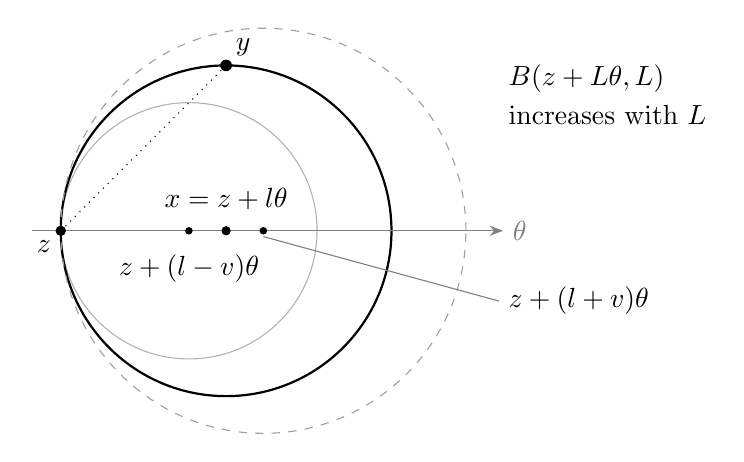
\begin{tikzpicture}[scale=1.05,>=Stealth]
 \draw[gray!60,thin] (1.55,0) circle[radius=1.55];
 \draw[black,thick] (2,0) circle[radius=2];
 \draw[gray!75,dashed] (2.45,0) circle[radius=2.45];
 \draw[->,gray] (-.35,0)--(5.35,0) node[right] {\(\theta\)};
 \fill (0,0) circle (1.8pt) node[below left] {\(z\)};
 \fill (1.55,0) circle (1.3pt) node[below=5pt] {\(z+(l-v)\theta\)};
 \fill (2,0) circle (1.6pt) node[above=4pt] {\(x=z+l\theta\)};
 \fill (2.45,0) circle (1.3pt);
 \draw[gray] (2.45,-.07)--(5.3,-.85)
   node[right,black] {\(z+(l+v)\theta\)};
 \fill (2,2) circle (2pt) node[above right] {\(y\)};
 \draw[dotted] (0,0)--(2,2);
 \node[align=left,anchor=west] at (5.3,1.65)
   {\(\displaystyle B(z+L\theta,L)\)\\[2pt]increases with \(L\)};
\end{tikzpicture}
\caption{The tangent-disk sweep. All boundary circles pass through \(z\).
A shell point \(y\) with \(|y-z|\ge\rho\) enters between the parameters
\(l-v\) and \(l+v\), with \(v\) proportional to
\(\delta/\rho^2\). Mass outside \(B(z,\rho)\) already present at
\(l-v\) lies in the inner disk \(B(x,l-2\delta)\). When
\(z\in D(x,r,\delta)\), this disk is contained in the controlled disk
\(B(x,r-\delta)\). The drawing is schematic.}
\label{fig:tangent-disks}
\end{figure}


For $z\in\R^2$ and $\theta$ on the unit circle define
\[
H_{z,\theta}(L)=
 \begin{cases}
 S\bigl(\{y:|y-z|\ge\rho\}\cap B(z+L\theta,L)\bigr),&L>0,\\
 0,&L\le0.
 \end{cases}
\]
This is bounded and nondecreasing in $L$. It is jointly Borel in all
its arguments, since it is the integral of the Borel indicator given
by \eqref{eq:shell-entry}, together with the other displayed tests.
For $l=|x-z|\in[1/2,3]$ and $\theta=(x-z)/l$, let $\mathcal C(x,z)$
be the condition
\begin{equation}\label{eq:shell-ray-condition}
H_{z,\theta}(l-v)\le T,
\qquad H_{z,\theta}(l+v)-H_{z,\theta}(l-v)\ge U.
\end{equation}
Define the nonnegative Borel function
\begin{align}
\mathcal M(x)=\frac1U\int_{1/2\le|x-z|\le3}
 \Bigg[&\frac1U\int
 \mathbf1_{\{\,\left||y-x|-|x-z|\right|\le2\delta,
                         \ |y-z|\ge\rho\,\}}\,d\nu(y)
 \notag\\[-2mm]
 &+\mathbf1_{\{\mathcal C(x,z)\}}\Bigg]\,d\nu(z),
 \qquad E=\{x:\mathcal M(x)\ge1\}.
 \label{eq:shell-majorant}
\end{align}

Suppose that \eqref{eq:shell-hypotheses} holds at $(x,r)$ and that
\eqref{eq:shell-cap} fails for every $z\in D=D(x,r,\delta)$.
For any such $z$, either
$\nu(D\setminus B(z,\rho))>U$ or
$S(D\setminus B(z,\rho))>U$.
Also $l=|x-z|\in[1/2,3]$ and every $y\in D$ satisfies
$\bigl||y-x|-l\bigr|\le2\delta$. In the first alternative, the
first term in brackets in \eqref{eq:shell-majorant} exceeds one.
In the second alternative, \eqref{eq:shell-entry-window} gives the
second inequality in \eqref{eq:shell-ray-condition}. The first
inequality follows from \eqref{eq:shell-earlier-interior}, because
$l-2\delta\le r-\delta$. The bracket is therefore at least one for
every $z\in D$. Since $\nu(D)\ge U$, we obtain
$\mathcal M(x)\ge1$. This proves the required implication outside
the Borel set $E$, simultaneously for all $r$.

It remains to estimate $\int\mathcal M$. For fixed $y,z$ with
$|y-z|\ge\rho$, the centers in the first term satisfy $|x-z|\le3$
and
\[
\bigl||x-y|^2-|x-z|^2\bigr|\le13\delta.
\]
The difference of squares is an affine function of $x$ with gradient
of length $2|y-z|$. These centers lie in a strip of width at most
$13\delta/|y-z|$ intersected with $\overline B(z,3)$, and thus have area at
most $C\delta/\rho$. Tonelli's theorem bounds the first contribution
to $\int\mathcal M$ by
$C\nu(\R^2)^2\delta/(U^2\rho)$.

For the second contribution, fix $z,\theta$ and abbreviate
$H=H_{z,\theta}$ and $G=\min(H,T+U)$. On the set of $l$ satisfying
\eqref{eq:shell-ray-condition},
\[
G(l+v)-G(l-v)\ge U.
\]
Because $G$ is bounded and nondecreasing,
\[
\int_{\R}\bigl(G(l+v)-G(l-v)\bigr)\,dl\le2v(T+U).
\]
For completeness, integration over $[-M,M]$ cancels the overlapping
intervals and leaves two intervals of length $2v$; letting $M$ increase
proves the inequality. Thus the permitted $l$ have length at most
$2v(1+T/U)$. Polar coordinates about $z$, with $l\le3$, and another
application of Tonelli's theorem bound the second contribution by
$C\nu(\R^2)v(1+T/U)/U$. Since $|E|\le\int\mathcal M$, these two
estimates prove \eqref{eq:shell-exception}.
\end{proof}


Under its shell and inner-disk mass hypotheses, the shell lemma
supplies a cap for every radius at a center outside one Borel set. The affine identity then suppresses the mass on that
cap. To obtain the discounted estimates, we still have to compare
kernel widths, control the positive interior mass in the directional
argument, and treat radii forced at band endpoints. We do this next;
the value estimate will require a separate kernel.

\subsection{Cancellation of small error pieces}

We now compare kernels at dyadic widths. Put
\begin{equation}\label{eq:local-exponents}
b=2\alpha=\frac1{50},\qquad
\eta=\frac1{10},\qquad \gamma=\frac15,
\qquad \delta_j=2^{-j}.
\end{equation}
Choose a fixed $\delta_*>0$ so small that $\delta_*\le1/4$ and
$\delta\le\delta^{2\gamma}/1600$ whenever $0<\delta\le\delta_*$.

We record estimates valid for any sequence of probability-mixture
kernels $K_j$, centered at the same $x$ and $r\in[1,2]$, with the
support and Lipschitz properties of Lemma~\ref{lem:local-balanced} at
width $\delta_j$. The zero-moment condition is not needed for these
estimates. Write
\begin{equation}\label{eq:local-coarse-measure}
\nu_j=\sum_{s_d\ge\delta_j^2}|\beta_d|,
\qquad p_j=\int K_j\,d\beta,
\qquad D_j=D(x,r,\delta_j).
\end{equation}
Then
\begin{equation}\label{eq:local-basic-cancellation}
\nu_j(\R^2)\le A\delta_j^{-b},
\qquad |p_j|\le C A\delta_j^{-\alpha}.
\end{equation}
Indeed, for $s_d<1$, subtracting the value of $K_j$ at the center of
a supporting ball gives
\[
\left|\int K_j\,d\beta_d\right|
 \le C m_d\min(1,s_d/\delta_j).
\]
For $s_d=1$, the same upper bound holds directly from $|K_j|\le1$.
Now use $\min(1,a)\le a^\alpha$ for $a>0$ and the definition of $A$.
The bound for $\nu_j$ follows directly from $s_d\ge\delta_j^2$.

If $F$ is a scalar or complex test function with
$\Lip(F)\le C/\delta_j$, the pieces with $s_d<\delta_j^2$ satisfy
\begin{equation}\label{eq:local-fine-cancellation}
\left|\sum_{s_d<\delta_j^2}\int F\,d\beta_d\right|
 \le \frac{C}{\delta_j}\sum_{s_d<\delta_j^2}s_dm_d
 \le C A\delta_j^{1-b}.
\end{equation}
Only the Lipschitz bound is used here; constants cancel because each
of these pieces has zero total vector mass. In particular,
\eqref{eq:local-fine-cancellation} applies to $K_{j+1}-K_j$ and to
$\overline{y-x}(K_{j+1}-K_j)$. These tests have the required global
Lipschitz bounds, since their supports are in $B(x,3)$.
Their supports are also in $D_j$. Consequently
\begin{align}
|p_{j+1}-p_j|
&\le C\bigl(\nu_j(D_j)+A\delta_j^{1-b}\bigr),
\notag\\
\left|\int\overline{y-x}(K_{j+1}-K_j)\,d\beta(y)\right|
&\le C\bigl(\nu_j(D_j)+A\delta_j^{1-b}\bigr).
\label{eq:local-increment-tests}
\end{align}

All these kernels are supported in $\Omega$ when $x\in Q$. Thus
\eqref{eq:local-decomposition} can be used in every pairing below,
even if some of its component measures have support outside $\Omega$.
For fixed $x,r$, as $j\to\infty$ the kernels converge off the circle
to $K_\infty=\mathbf1_{B(x,r)}$. Absolute continuity of all the
component measures gives convergence of their integrals by dominated
convergence. The same holds for the moment integrals. In particular, if every
finite-width kernel is balanced, then $K_\infty$ has zero moment as
well. This is a statement at each fixed $(x,r)$: every circle has zero
mass for every absolutely continuous component. There is no exceptional
set depending on the radius to remove. Absolute continuity is used
here, but was not needed in the Borel shell lemma.

\subsection{The directional estimate}

We now prove \eqref{eq:local-direction}. If $A=0$, all the error
measures vanish, and $e\cdot h(B(x,r))\ge0$ for every relevant disk;
the conclusion follows. Assume $A>0$.

We prove a superlevel-set estimate by separating widths at which the
coarse error mass in the shell is small from those at which it is large.
Small-mass widths have directly summable error increments. At the
remaining widths we compare only increases of the negative projection:
the later negative projection controls the interior positive mass,
allowing Lemma~\ref{lem:shell-concentration} to be applied.

Let $\lambda\ge L_0A$, where the fixed constant $L_0$ will be chosen
large enough in the course of the proof. Put $q=A/\lambda$ and choose
$j_0$ so that
\begin{equation}\label{eq:local-start-scale}
q/2<\delta_{j_0}\le q.
\end{equation}
We require $L_0\ge1/\delta_*$, so all widths under consideration are
at most $\delta_*$. At a fixed $x\in Q$ and $r\in\mathcal I(x)$,
use Lemma~\ref{lem:local-balanced} to choose $K_j$ for every
$j\ge j_0$, and write
\[
P_j=\int K_j\,dh,
\qquad N_j=(-e\cdot P_j)_+,
\qquad U_j=\lambda\delta_j^\eta.
\]
Call $j$ active for $(x,r)$ if $\nu_j(D_j)\ge U_j$.
If it is inactive, \eqref{eq:local-increment-tests} and
$1-b>\eta$ give
\begin{equation}\label{eq:local-inactive}
|p_{j+1}-p_j|
+\left|\int\overline{y-x}(K_{j+1}-K_j)\,d\beta(y)\right|
 \le C\lambda\delta_j^\eta.
\end{equation}
Here and below we use $A\le\lambda$.

Choose $C_0$ sufficiently large depending only on $C_s$ and $\kappa$,
and put $T_j=C_0\lambda\delta_j^{-b}$. Apply
Lemma~\ref{lem:shell-concentration} with
\[
\nu=\nu_j,\quad \delta=\delta_j,\quad
\rho=\delta_j^\gamma,\quad U=U_j,\quad T=T_j.
\]
It gives Borel sets $E_j$, independent of $r$, such that
\begin{equation}\label{eq:local-shell-tail}
|E_j|\le C\left[
q^2\delta_j^{14/25}+q\delta_j^{9/25}\right].
\end{equation}
To check the exponents, the first term of
\eqref{eq:shell-exception} gives
$1-\gamma-2b-2\eta=14/25$. The second term is a sum of powers
$1-2\gamma-b-\eta$ and $1-2\gamma-2b-2\eta=9/25$; because
$\delta_j\le1$, both are bounded by a constant times the latter.
Constants in \eqref{eq:local-shell-tail} may depend on the already
fixed $C_0$.

Fix a center outside $\bigcup_{j\ge j_0}E_j$, and keep any
$r\in\mathcal I(x)$ fixed. Positivity in the direction $e$ implies
\begin{equation}\label{eq:local-cone-sign}
e\cdot P_j\ge\kappa\int K_j\,dS+e\cdot p_j,
\qquad N_j\le|p_j|.
\end{equation}
Before the first active index, all the increments of $p_j$ obey
\eqref{eq:local-inactive}. Hence, if $j$ is the first active index,
or if $j=\infty$ and there are no active indices,
\begin{equation}\label{eq:local-first-active}
N_j\le C\left(A\delta_{j_0}^{-\alpha}
                   +\lambda\delta_{j_0}^\eta\right).
\end{equation}
The formula at infinity follows from the dominated-convergence
observation above.

The first active width has therefore been controlled. To continue,
we compare consecutive active widths, allowing arbitrarily many
inactive widths between them. Only an increase of the negative
projection needs a new estimate; that sign will supply the positive
interior-mass bound required by the shell lemma.

Suppose now that $j$ is active and $l>j$ is the next active index;
set $l=\infty$ if there is no next one. The individual bound in
\eqref{eq:local-basic-cancellation} at $j$ and $j+1$, followed by
the inactive increments between $j+1$ and $l$, gives
\begin{equation}\label{eq:local-gap-errors}
|p_j|+|p_l|
 \le C\left(A\delta_j^{-\alpha}
                  +\lambda\delta_j^\eta\right)
 \le C\lambda\delta_j^{-b}.
\end{equation}
We need to estimate a change only when $N_l>N_j$. In that case
$e\cdot P_l<0$, so \eqref{eq:local-cone-sign} gives
\[
\int K_l\,dS\le\kappa^{-1}|p_l|.
\]
Since $K_l=1$ on $B(x,r-\delta_j)$, this proves
$S(B(x,r-\delta_j))\le T_j$ after fixing $C_0$ large enough to
dominate the constant just obtained. The shell lemma therefore
supplies a point $z\in D_j$ such that
\begin{equation}\label{eq:local-chosen-cap}
(S+\nu_j)\bigl(D_j\setminus B(z,\delta_j^\gamma)\bigr)
 \le2U_j.
\end{equation}
This point is used only at the current center and radius; no
measurable selection of $z$ is required.

To estimate the positive mass on the cap, we need a weighted bound
for both kernels being compared. The sign at $l$ supplies one, but
$e\cdot P_j>0$ would give no corresponding bound for $K_j$.
We therefore replace $K_j$, when necessary, by a kernel with zero
projection and the same negative part.
If $e\cdot P_j\le0$, set $K_*=K_j$. Otherwise, interpolate between
$K_j$ and $K_l$ to obtain a convex combination $K_*$ with
$e\cdot P_*=0$, where $P_* =\int K_*\,dh$. This is possible because
$e\cdot P_l<0$. In either case,
\[
N_*:=(-e\cdot P_*)_+=N_j,
\qquad e\cdot P_*\le0.
\]
Writing $p_* =\int K_*\,d\beta$ and using
\eqref{eq:local-gap-errors} and \eqref{eq:local-cone-sign}, we get
\begin{equation}\label{eq:local-weighted-good}
\int(K_l+K_*)\,dS\le C\lambda\delta_j^{-b}.
\end{equation}

All of $K_j,K_l,K_*$ have zero moment, including when $l=\infty$
by the preceding sharp-kernel limit. Since $|z-x|\ge1/2$, define
\[
W(y)=1-\frac{\overline{y-x}}{\overline{z-x}}.
\]
The affine identity in Lemma~\ref{lem:local-affine} gives
\begin{equation}\label{eq:local-corrected-difference}
P_l-P_* =\int W(y)(K_l-K_*)(y)\,dh(y).
\end{equation}
The difference of kernels is supported on $D_j$, and
\[
|W|\le C\delta_j^\gamma\quad\hbox{on }B(z,\delta_j^\gamma),
\qquad |W|\le C\quad\hbox{on }D_j.
\]
The contribution of $\sum_i v_i\sigma_i$ to
\eqref{eq:local-corrected-difference} is therefore at most
\begin{equation}\label{eq:local-good-cap-cost}
C\lambda\delta_j^{\gamma-b}+C U_j,
\end{equation}
by \eqref{eq:local-weighted-good},
$|K_l-K_*|\le K_l+K_*$, and \eqref{eq:local-chosen-cap}.

For the error measures, $K_l-K_*$ is a scalar multiple in $[0,1]$
of $K_l-K_j$. Keep $W$ fixed and telescope
\begin{equation}\label{eq:local-error-telescoping}
\int W(K_l-K_j)\,d\beta
 =\sum_{i=j}^{l-1}\int W(K_{i+1}-K_i)\,d\beta.
\end{equation}
For $l=\infty$ this equality means the limit of the finite sums.
We never apply a Lipschitz cancellation bound directly to the sharp
kernel $K_\infty$ or to its interpolant: only the finite consecutive
differences in this sum need such a bound.
On the first step, the pieces contributing to $\nu_j$ cost at most
$C\delta_j^\gamma\nu_j(\R^2)+CU_j$ by
\eqref{eq:local-chosen-cap}. The remaining pieces cost
$CA\delta_j^{1-b}$ by \eqref{eq:local-fine-cancellation}, since
$W(K_{j+1}-K_j)$ has Lipschitz constant at most $C/\delta_j$.
For $j<i<l$, use
\[
\int W(K_{i+1}-K_i)\,d\beta
 =p_{i+1}-p_i-\frac1{\overline{z-x}}
       \int\overline{y-x}(K_{i+1}-K_i)\,d\beta(y).
\]
These are inactive steps, so their absolute values sum to at most
$C\lambda\delta_j^\eta$ by \eqref{eq:local-inactive}.
Combining the estimates gives
\[
\left|\int W(K_l-K_j)\,d\beta\right|
 \le C\left(A\delta_j^{\gamma-b}
       +A\delta_j^{1-b}+\lambda\delta_j^\eta\right).
\]
Together with \eqref{eq:local-good-cap-cost}, and using
$\gamma-b=9/50>\eta$, this yields
\begin{equation}\label{eq:local-active-increment}
N_l\le N_j+|P_l-P_*|\le N_j+C\lambda\delta_j^\eta.
\end{equation}
The same inequality is automatic when $N_l\le N_j$.

Sum \eqref{eq:local-active-increment} along the active indices. If
there are finitely many, include the last comparison with $l=\infty$;
if there are infinitely many, pass to the limit along them. Dominated
convergence and \eqref{eq:local-first-active} give
\begin{equation}\label{eq:local-final-projection}
(-e\cdot h(B(x,r)))_+
 \le C\left(A\delta_{j_0}^{-\alpha}
                   +\lambda\delta_{j_0}^\eta\right)
 \le C\lambda\left(q^{1-\alpha}+q^\eta\right).
\end{equation}
This holds for every $r\in\mathcal I(x)$ at the fixed center outside
the exceptional sets. Increase $L_0$, depending only on $C_s$ and
$\kappa$, so that the last bound is less than $\lambda$ whenever
$q\le L_0^{-1}$.

Let $Y(x)=\sup_{r\in\mathcal I(x)}(-e\cdot h(B(x,r)))_+$.
Summing \eqref{eq:local-shell-tail} and using
\eqref{eq:local-start-scale}, we have proved
\begin{equation}\label{eq:local-direction-tail}
|\{x\in Q:Y(x)>\lambda\}|
 \le C\left[
       (A/\lambda)^{64/25}+(A/\lambda)^{34/25}\right]
 \qquad(\lambda\ge L_0A).
\end{equation}
Both powers exceed one. The layer-cake formula, the trivial bound
$|Q|=1$ for smaller thresholds, and the substitution
$\lambda=As$ give
\[
\int_QY\,dx
 \le L_0A+C A\int_{L_0}^{\infty}
                  (s^{-64/25}+s^{-34/25})\,ds\le C A.
\]
Finally, \eqref{eq:local-spatial-gradient} and $r\ge1$ prove
\eqref{eq:local-direction}.

\subsection{The size estimate, including band endpoints}

To prove \eqref{eq:local-size}, place the measures $v_i\sigma_i$
among the error measures with assigned size one. The augmented price is
$A_{\mathrm{tot}}=A+S(\R^2)$, where $A$ and $S$ refer to the original
decomposition. The augmented positive part is zero; in this proof,
$\beta$ and $\nu_j$ refer to the augmented error family.
If $A_{\mathrm{tot}}=0$, the result is immediate.

Take $\lambda\ge L_0A_{\mathrm{tot}}$, put $q=A_{\mathrm{tot}}/\lambda$, and choose $j_0$ as in
\eqref{eq:local-start-scale}. Here $L_0$ will depend only on $C_s$. For $x\in Q$ and
$r\in\mathcal J(x)$, choose the balanced kernel $K_j$ when
$\dist(r,\{1,2\})\ge\delta_j$. Such an $r$ is an actual
maximizer on $[1,2]$, so the two neighboring radii needed in
Lemma~\ref{lem:local-balanced} are admissible. Otherwise choose the
uniform probability mixture over $[r-\delta_j,r+\delta_j]$.
The latter kernel need not have zero moment, but has all the same
support, positivity and Lipschitz bounds. Thus
\eqref{eq:local-basic-cancellation}--\eqref{eq:local-increment-tests}
remain valid with $A_{\mathrm{tot}}$ in place of $A$. Write $P_j=\int K_j\,dh=p_j$, and again call $j$
active when $\nu_j(D_j)\ge U_j=\lambda\delta_j^\eta$.

There is an additional Borel exceptional set for each width:
\begin{equation}\label{eq:local-endpoint-exception}
F_j=\bigcup_{a\in\{1,2\}}
 \left\{x:\nu_j\{y:\bigl||y-x|-a\bigr|\le2\delta_j\}
                         \ge U_j\right\}.
\end{equation}
For each fixed $y$, the areas of these two annuli of centers sum to
$24\pi\delta_j$. Tonelli's theorem and Markov's inequality give
\begin{equation}\label{eq:local-endpoint-area}
|F_j|\le24\pi\delta_j\frac{\nu_j(\R^2)}{U_j}
 \le C(A_{\mathrm{tot}}/\lambda)\delta_j^{22/25}.
\end{equation}
If $\dist(r,\{1,2\})<\delta_j$, the shell $D_j$ lies in one of
the annuli in \eqref{eq:local-endpoint-exception}. Thus, outside
$F_j$, an active index must satisfy
$\dist(r,\{1,2\})\ge\delta_j$, and both $K_j$ and $K_{j+1}$
have zero moment. In particular, the forced radii $r=1,2$ are
covered even if they are not maximizers.

Apply Lemma~\ref{lem:shell-concentration} with $S=0$, $T=0$,
$\nu=\nu_j$, $\delta=\delta_j$, $\rho=\delta_j^\gamma$, and $U=U_j$.
It supplies Borel exceptional sets $E_j$, independent of $r$, with bound
$C[q^2\delta_j^{14/25}+q\delta_j^{12/25}]$, which is at most the
right side of \eqref{eq:local-shell-tail}. Its constants have no cone
parameter: the positive measure and its interior-mass threshold are
both zero.
At an active step
outside $E_j\cup F_j$, its interior-mass hypothesis is automatic,
and it gives a point $z\in D_j$ with
$\nu_j(D_j\setminus B(z,\delta_j^\gamma))\le2U_j$.
The zero moments allow the correction
\[
P_{j+1}-P_j=\int
 \left(1-\frac{\overline{y-x}}{\overline{z-x}}\right)
 (K_{j+1}-K_j)(y)\,d\beta(y).
\]
The coarse pieces cost at most
$C A_{\mathrm{tot}}\delta_j^{\gamma-b}+CU_j$, and the fine pieces cost at most
$C A_{\mathrm{tot}}\delta_j^{1-b}$, exactly as above. Hence
\[
|P_{j+1}-P_j|\le C\lambda\delta_j^\eta.
\]
At an inactive step the same inequality follows directly from
\eqref{eq:local-increment-tests}, without using a moment identity.
Starting with $|P_{j_0}|\le CA_{\mathrm{tot}}\delta_{j_0}^{-\alpha}$ and summing
all increments, we obtain
\[
|h(B(x,r))|\le C\lambda(q^{1-\alpha}+q^\eta)<\lambda
\]
after increasing $L_0$. This holds simultaneously for all
$r\in\mathcal J(x)$ outside $\bigcup_{j\ge j_0}(E_j\cup F_j)$.
The measure bound is therefore
\begin{align}
\left|\left\{x\in Q:
       \sup_{r\in\mathcal J(x)}|h(B(x,r))|>\lambda\right\}\right|
 \le C\bigl[&(A_{\mathrm{tot}}/\lambda)^{64/25}
              +(A_{\mathrm{tot}}/\lambda)^{34/25}
 \notag\\[-1mm]
              &+(A_{\mathrm{tot}}/\lambda)^{47/25}\bigr].
\label{eq:local-size-tail}
\end{align}
Every exponent is larger than one. The same layer-cake computation
as before gives the unnormalized bound by $CA_{\mathrm{tot}}$. Since
$A_{\mathrm{tot}}=A+S(\R^2)$,
\eqref{eq:local-spatial-gradient} proves \eqref{eq:local-size}.

\subsection{The value-oscillation estimate}

This estimate involves all small radii and does not use a maximizing
property. We express $g$ minus a fixed mean through its gradient,
prove an $L^{3/2}$ cancellation bound for the resulting kernel, and
then apply the strong maximal inequality.

We finish the proof of Lemma~\ref{lem:local} by establishing
\eqref{eq:local-value}. Choose a nonnegative smooth probability
density $\psi$ supported in the interior of $Q$, with uniformly
bounded derivatives after translating and rotating a fixed choice,
and put
\[
c=\int g(z)\psi(z)\,dz,
\qquad E_Q=\{x:\dist(x,Q)<4\}.
\]
For $x\in E_Q$, integrate $\nabla g$ along the segments from $x$
to points of $\supp\psi$ and change variables to obtain
\begin{equation}\label{eq:local-value-kernel}
g(x)-c=\int L(x,y)\cdot dh(y),
\qquad
L(x,y)=-(y-x)\int_0^1
              \psi\bigl(x+(y-x)/t\bigr)t^{-3}\,dt.
\end{equation}
Indeed, this is the fundamental theorem of calculus in
$g(x)-g(z)=-\int_0^1(z-x)\cdot\nabla g(x+t(z-x))\,dt$,
followed by $y=x+t(z-x)$.

The displayed formula defines $L(x,y)$ for every $y\ne x$ in
the plane, not only for $y\in\Omega$. This global definition will
allow cancellation against a support center outside $\Omega$.
For each fixed $x\in E_Q$, the kernel is supported on segments
joining $x$ to $\supp\psi$, and hence is supported in $\Omega$.
It is smooth in $y\ne x$, with the uniform bounds
\begin{equation}\label{eq:local-value-kernel-bounds}
|L(x,y)|\le\frac{C}{|x-y|},
\qquad |\nabla_yL(x,y)|\le\frac{C}{|x-y|^2}.
\end{equation}
To verify them, if the integrand or one of its derivatives is
nonzero, then $|y-x|\le Ct$, since $x\in E_Q$ and
$x+(y-x)/t$ lies in a fixed bounded neighborhood of $Q$.
The first bound follows by integrating $t^{-3}$ from
$|y-x|/C$ to one and multiplying by $|y-x|$. Differentiation in
$y$ produces either the same integral or
$|y-x|\int t^{-4}\,dt$, which gives the second bound.

Fix $p=3/2$, so $2/p-1=1/3>\alpha$. The first bound in
\eqref{eq:local-value-kernel-bounds} implies
\begin{equation}\label{eq:local-kernel-lp}
\sup_{y\in\R^2}\|L(\cdot,y)\|_{L^p(E_Q)}\le C.
\end{equation}
This follows by integrating $|x-y|^{-p}$ on a bounded set;
$p<2$ makes the singularity integrable, uniformly in $y$.

Consider a piece $\beta_d$ with $s_d<1$, supported in
$B(z,a)$, where we may take $a=C_s s_d$ after increasing $C_s$
to at least one. On $E_Q\cap B(z,2a)$, the first kernel bound and
Minkowski's inequality give
\[
\left\|\int L(\cdot,y)\cdot d\beta_d(y)\right\|_
                       {L^p(E_Q\cap B(z,2a))}
 \le C a^{2/p-1}m_d.
\]
In fact, for $y\in B(z,a)$ the relevant $x$ lie within $3a$ of
$y$, and the $L^p$ norm of $|x-y|^{-1}$ there is
$C a^{2/p-1}$.
For $|x-z|>2a$, use the zero total vector mass to subtract
$L(x,z)$. The derivative bound in
\eqref{eq:local-value-kernel-bounds}, applied on the segment from
$z$ to $y$, gives
\[
\left|\int L(x,y)\cdot d\beta_d(y)\right|
 \le C a m_d|x-z|^{-2}.
\]
Its $L^p$ norm on $\{|x-z|>2a\}$ is at most
$C a^{2/p-1}m_d$, since $p>1$. Combining the two regions yields
\begin{equation}\label{eq:local-value-piece}
\left\|\int L(\cdot,y)\cdot d\beta_d(y)\right\|_{L^p(E_Q)}
 \le C s_d^{1/3}m_d\le C s_d^\alpha m_d.
\end{equation}
The constant may depend on $C_s$. For a piece of assigned size
one, and for the positive measures, use
\eqref{eq:local-kernel-lp} directly. Minkowski's inequality and the
finite decomposition therefore give
\begin{equation}\label{eq:local-value-lp}
\|g-c\|_{L^{3/2}(E_Q)}\le C\bigl(A+S(\R^2)\bigr).
\end{equation}
These same estimates show that the integrals obtained by inserting
\eqref{eq:local-decomposition} into \eqref{eq:local-value-kernel}
exist for almost every $x$; thus the use of the potentially singular
kernel is justified.

Let $f_Q=(g-c)\mathbf1_{E_Q}$, extended by zero to the plane.
Every disk centered at $x\in Q$ of radius at most four is contained
in $E_Q$. Consequently
\[
\sup_{0<t,t'\le4}|u_t(x)-u_{t'}(x)|\le2Mf_Q(x),
\]
where the maximal function on the right uses absolute values.
The classical strong $L^{3/2}$ maximal inequality
\cite[(1.2)]{Kinnunen1997}, followed by H\"older's inequality on the unit square and
\eqref{eq:local-value-lp}, proves \eqref{eq:local-value}. This
completes the proof of Lemma~\ref{lem:local}.

\section{Dyadic vector masses and common prices}
\label{sec:prices}

Throughout this section, let $g\in C_c^\infty(\R^2)$ be real valued, and write
\[
 h=\nabla g\,\dd x,
 \qquad V=|h|(\R^2),
 \qquad u_t=A_tg.
\]
The averages $u_t$ are signed. Fix an integer $m\ge1$; all estimates below
are uniform in $m$.
Lemma~\ref{lem:local} discounts a cancelling error according to the
size of its support. We now decompose the gradient into errors to which
that discount applies, and assign one summable price to each dyadic
cell. The same price will work for every direction in a fixed finite
palette. The construction starts with the actual density of each scalar
coordinate of the gradient at the finest level and removes equal positive
and negative masses as it moves toward coarser levels.

\subsection{Positive refinement and cone coordinates}

For every integer $k$, set $r_k=2^{-k}$ and $V_k=r_k\mathbb Z^2$.
These definitions are not restricted to $1,\ldots,m$: the neighboring
direction estimate in Section~\ref{sec:labels} will also use level
$k-12$.
A vertex includes its level, so vertices at different levels are distinct
even when their spatial positions agree. For $p\in V_k$, define
\[
 Q_p=p+[0,r_k)^2,
 \qquad
 \phi_p(x)=\prod_{j=1}^2
       \left(1-\frac{|x_j-p_j|}{r_k}\right)_+.
\]
For $p\in V_i$ and $q\in V_k$ with $i<k$, put
$\lambda_{pq}=\phi_p(q)$, and at equal levels put
$\lambda_{pq}=\mathbf 1_{\{p=q\}}$. These nonnegative coefficients satisfy
\begin{equation}
\begin{gathered}
 \sum_{p\in V_i}\lambda_{pq}=1,
 \qquad
 \phi_p=\sum_{q\in V_k}\lambda_{pq}\phi_q
 \quad (i\le k),
 \\
 \lambda_{ps}=\sum_{q\in V_j}\lambda_{pq}\lambda_{qs}
 \quad (i\le j\le k,\ p\in V_i,\ s\in V_k).
\end{gathered}
\label{eq:hat-refinement}
\end{equation}
To verify these identities, first consider one coordinate. The hats on a
fixed grid sum to one: between two consecutive vertices, the only nonzero
hats have complementary affine values. A coarse hat is affine on every
interval of any finer dyadic grid, since all its breakpoints belong to
that grid. It therefore equals the piecewise affine interpolant of its
values at the finer vertices. Taking products proves the first two
identities in \eqref{eq:hat-refinement}; evaluating the second identity at
$s$ proves the third. The sums are locally finite. Notice that the normalization is in
the coarse index $p$ for each fixed fine vertex $q$. These coefficients
are refinement weights, not stochastic transition rows.

If $q\in V_{k+1}$ and $\lambda_{pq}>0$, then in each coordinate
$q_j-p_j\in\{-r_k/2,0,r_k/2\}$. Consequently
\begin{equation}
 \supp\phi_q\subseteq\supp\phi_p.
 \label{eq:prices-support-nesting}
\end{equation}
Thus each vertex has nine positive-weight children, and the supports
remain nested along every path of positive-weight edges.

Define the vector masses and their polar decompositions by
\[
 h_p=\int\phi_p\,\dd h,
 \qquad a_p=|h_p|,
 \qquad h_p=a_p\theta_p,
\]
where $\theta_p$ is an arbitrary fixed unit vector when $a_p=0$.
Refinement gives
\[
 h_p=\sum_{q\in V_k}\lambda_{pq}h_q
 \quad(p\in V_i,\ i\le k).
\]
The triangle inequality and the column sums in
\eqref{eq:hat-refinement} imply
\begin{equation}
 \sum_{p\in V_i}a_p
 \le\sum_{q\in V_k}a_q
 \le V
 \quad(i\le k).
 \label{eq:prices-vector-mass-budget}
\end{equation}
The last inequality follows directly from $\sum_q\phi_q=1$.
At each fixed level only finitely many of these masses can be nonzero,
because $h$ has compact support.

Fix $\tau=1/100$ and a finite $\tau/20$-net $\mathcal N$ of the unit
circle, measured in chord distance. For $n\in\mathcal N$, let $n^\perp$
be its counterclockwise quarter turn and put
\[
 e_+(n)=\frac{\sqrt3}{2}n+\frac12n^\perp,
 \qquad
 e_-(n)=\frac{\sqrt3}{2}n-\frac12n^\perp.
\]
These are unit vectors and $e_+(n)\cdot e_-(n)=1/2$.
Call $(q,n)$ \emph{good} when $\theta_q$ belongs to the closed sector
between $e_-(n)$ and $e_+(n)$, and \emph{bad} otherwise.
The two scalar coefficient functionals
\begin{equation}
 c_{n,+}(z)=\frac{n\cdot z}{\sqrt3}+n^\perp\cdot z,
 \qquad
 c_{n,-}(z)=\frac{n\cdot z}{\sqrt3}-n^\perp\cdot z
 \label{eq:prices-scalar-coordinates}
\end{equation}
satisfy
\[
 z=e_+(n)c_{n,+}(z)+e_-(n)c_{n,-}(z),
 \qquad
 |c_{n,+}(z)|+|c_{n,-}(z)|
 =2\max\left\{\frac{|n\cdot z|}{\sqrt3},
                     |n^\perp\cdot z|\right\}
 \le2|z|.
\]
In particular, for a good pair $(q,n)$, both coefficients of $h_q$ are
nonnegative, including when $h_q=0$. This sign information will supply
the positive cone measures in Lemma~\ref{lem:local}.

For the finite-band assembly, we also need to bound a vector's norm
by its signed projection along $n$ and the unfavorable projections
controlled by the local estimate. The following inequality gives
that bound, with an absolute constant:
\begin{equation}
 |z|\le C\left(n\cdot z+
                \sum_{\varepsilon\in\{+,-\}}
                (-e_\varepsilon(n)\cdot z)_+\right)
 \quad(z\in\R^2).
 \label{eq:cone-algebra}
\end{equation}
Here the expression in parentheses is nonnegative. Indeed, writing
$a=n\cdot z$, its value is positive for every nonzero $z$: if $a>0$
this is immediate; if $a=0$, one of the two negative parts equals
$|z|/2$; and if $a<0$, their sum is at least
$-(e_+(n)+e_-(n))\cdot z=\sqrt3|a|$, so the expression is at least
$(\sqrt3-1)|a|>0$. Its minimum on the unit circle is therefore positive
by continuity. Rotation invariance makes this minimum independent of
$n$, and homogeneity proves \eqref{eq:cone-algebra}.

\subsection{Cancellation from the finest level upward}

Let $\mathcal C$ be the indexed finite family consisting of
$c_{n,+},c_{n,-}$ for every $n\in\mathcal N$; repeated functionals,
if any, retain their indices. For $c\in\mathcal C$ write
\[
 \nu^c=c(h)=c(\nabla g(x))\,\dd x,
 \qquad c_s=c(h_s)=\int\phi_s\,\dd\nu^c.
\]
For $s\in V_l$, $1\le l\le m$, define
\begin{equation}
 d_s^c=
 \begin{cases}
 \displaystyle\frac12\left(
       \sum_{t\in V_{l+1}}\lambda_{st}|c_t|-|c_s|\right),
       & l<m,\\[6pt]
 \displaystyle\frac12\left(
       \int\phi_s(x)|c(\nabla g(x))|\,\dd x-|c_s|\right),
       & l=m.
 \end{cases}
 \label{eq:prices-scalar-defects}
\end{equation}
These numbers are nonnegative by refinement and the triangle
inequality. They measure the equal positive and negative masses
that can be removed at $s$. At level $m$ the definition uses the
positive and negative parts of the density itself. In particular,
$c_s=0$ need not imply $d_s^c=0$.

We will realize this numerical cancellation by measures supported
in the corresponding tent. The elementary operation
is proportional removal; it does not require the two measures
being paired to be mutually singular.

\begin{lemma}[Removing equal masses]\label{lem:prices-remove}
Let $U,V$ be finite nonnegative measures, of masses $P,N$.
There are nonnegative submeasures $\mu_+\le U$, $\mu_-\le V$,
both of mass $d=\min(P,N)$, such that
\[
 U-V=\rho+\mu_+-\mu_-,\qquad
 \rho(\R^2)=P-N,\qquad |\rho|(\R^2)=|P-N|.
\]
The residual $\rho$ has constant sign. If $U,V$ are absolutely
continuous and supported in a common closed set, so are all the
constructed measures.
\end{lemma}
\begin{proof}
When $P>0$ set $\mu_+=(d/P)U$; when $P=0$ set $\mu_+=0$.
Define $\mu_-$ in the same way from $N,V$, and set
$\rho=(U-\mu_+)-(V-\mu_-)$. If $P\ge N$ and $P>0$, then
$\mu_-=V$ and $\rho=(1-N/P)U\ge0$. The case $N\ge P$ is
symmetric. If $P=N=0$, every measure is zero. These formulas
prove the mass, sign and support assertions, including all zero
cases.
\end{proof}

\begin{lemma}[Exact scalar pairing]\label{lem:prices-scalar-pairing}
For every $c\in\mathcal C$ there are measures
$\rho_s^c,\mu_{s,+}^c,\mu_{s,-}^c$ at all vertices
$s\in V_l$, $1\le l\le m$, supported in $\supp\phi_s$ and
absolutely continuous, with $\rho_s^c$ of constant sign and
$\mu_{s,\pm}^c$ nonnegative, such that
\begin{equation}\label{eq:prices-scalar-masses}
 \rho_s^c(\R^2)=c_s,\qquad |\rho_s^c|(\R^2)=|c_s|,
 \qquad
 \mu_{s,+}^c(\R^2)=\mu_{s,-}^c(\R^2)=d_s^c.
\end{equation}
Put $\beta_s^c=\mu_{s,+}^c-\mu_{s,-}^c$. For every
$q\in V_k$, $1\le k\le m$, the following is an identity of
measures on the whole plane:
\begin{equation}\label{eq:prices-vertex-reconstruction}
 \phi_q\nu^c=\rho_q^c+
       \sum_{l=k}^m\sum_{s\in V_l}\lambda_{qs}\beta_s^c.
\end{equation}
Only finitely many terms in this identity are nonzero, and
\begin{equation}\label{eq:prices-pair-properties}
 \beta_s^c(\R^2)=0,\qquad
 |\beta_s^c|(\R^2)\le2d_s^c,\qquad
 \supp\beta_s^c\subseteq\supp\phi_s
       \subseteq\overline B(s,\sqrt2 r_l).
\end{equation}
\end{lemma}

\begin{proof}
Fix $c$ and first take $s\in V_m$. Apply
Lemma~\ref{lem:prices-remove} to the actual terminal measures
\[
 U_s=\phi_s(\nu^c)_+,
 \qquad V_s=\phi_s(\nu^c)_-.
\]
Their masses have difference $c_s$ and sum
$\int\phi_s\,\dd|\nu^c|$. Hence their smaller mass is exactly
$d_s^c$, and removal gives \eqref{eq:prices-scalar-masses} and
\begin{equation}\label{eq:prices-terminal-identity}
 \phi_s\nu^c=\rho_s^c+\beta_s^c.
\end{equation}
If the positive and negative terminal masses agree, the residual
is zero while both paired measures keep that common mass.

Suppose that all residuals at level $l+1$ have been constructed.
At $s\in V_l$ combine their positive and negative parts separately:
\[
 U_s=\sum_{t\in V_{l+1}}\lambda_{st}(\rho_t^c)_+,
 \qquad
 V_s=\sum_{t\in V_{l+1}}\lambda_{st}(\rho_t^c)_-.
\]
The residuals have constant sign, so the masses $P_s,N_s$ of
these two measures obey
\[
 P_s-N_s=\sum_t\lambda_{st}c_t=c_s,
 \qquad
 P_s+N_s=\sum_t\lambda_{st}|c_t|.
\]
Thus $\min(P_s,N_s)=d_s^c$. Applying
Lemma~\ref{lem:prices-remove} again constructs the measures in
\eqref{eq:prices-scalar-masses} and proves
\begin{equation}\label{eq:prices-residual-recursion}
 \sum_{t\in V_{l+1}}\lambda_{st}\rho_t^c
      =\rho_s^c+\beta_s^c.
\end{equation}
Absolute continuity is preserved by finite sums and scalar
multiplication. Support nesting in
\eqref{eq:prices-support-nesting} keeps all these measures in
$\supp\phi_s$. The construction proceeds through finitely many
levels. At each level only finitely many measures can be nonzero,
since the terminal density has compact support and each vertex
has finitely many parents.

It remains to verify that no density has been lost during removal.
At level $m$, \eqref{eq:prices-vertex-reconstruction} is
\eqref{eq:prices-terminal-identity}. If the identity holds for
all children of $q\in V_k$, refinement yields
\begin{align*}
 \phi_q\nu^c
 &=\sum_{t\in V_{k+1}}\lambda_{qt}\phi_t\nu^c\\
 &=\sum_t\lambda_{qt}\rho_t^c
   +\sum_{l=k+1}^m\sum_{s\in V_l}
        \left(\sum_t\lambda_{qt}\lambda_{ts}\right)\beta_s^c\\
 &=\rho_q^c+\beta_q^c
   +\sum_{l=k+1}^m\sum_{s\in V_l}\lambda_{qs}\beta_s^c.
\end{align*}
The last line uses \eqref{eq:prices-residual-recursion} and
coefficient composition in \eqref{eq:hat-refinement}. It is the
required identity at $q$. All rearrangements are finite for a
fixed root because branching and depth are finite. Finally,
equal masses in \eqref{eq:prices-scalar-masses} give zero mass
and variation at most $2d_s^c$ for each difference; the tent
support gives the last assertion in
\eqref{eq:prices-pair-properties}.
\end{proof}

The measures are constructed once at each vertex. A descendant's
pair may appear in several coarse identities, with its specified
coefficient; these identities do not assert a disjoint allocation.

\paragraph{The equivalent path form.}
The price estimate below uses the vertex identity. The following
equivalent form expresses shared-descendant coefficients as sums of
path weights, using the same cancelling pieces. Section~\ref{sec:labels}
will construct a separate positive measure on vector paths. Fix $q\in V_k$ with $1\le k\le m$, and let $\xi$ range
over all positive-weight paths $\xi=(q_k,\ldots,q_l)$ with
$q_k=q$ and $k\le l\le m$, including the trivial path $(q)$. Set
\[
 w_\xi=\prod_{j=k}^{l-1}\lambda_{q_jq_{j+1}},
 \qquad \mu_{\xi,\pm}^c=w_\xi\mu_{q_l,\pm}^c,
 \qquad w_{(q)}=1.
\]
Composition gives $\sum_{\xi:q_l=s}w_\xi=\lambda_{qs}$, and
therefore
\begin{equation}\label{eq:prices-scalar-pairing}
 \phi_q c(h)=\rho_q^c+
       \sum_\xi(\mu_{\xi,+}^c-\mu_{\xi,-}^c).
\end{equation}
Each path pair has mass $w_\xi d_s^c$ in each sign and support in
$\supp\phi_s$, where $s=q_l$. This recovers the path identity
without a separate allocation along every path.

The cancellation amounts have an exact total budget. Summing
\eqref{eq:prices-scalar-defects} over a level and using the column
normalization in \eqref{eq:hat-refinement} cancels intermediate
absolute masses. The terminal partition of unity gives
\begin{equation}
 \sum_{l=1}^m\sum_{s\in V_l}d_s^c
 =\frac12\left(
       \int|c(\nabla g)|\,\dd x-
       \sum_{s\in V_1}|c_s|\right)
 \le\frac12\|c\|\,V.
 \label{eq:prices-scalar-defect-budget}
\end{equation}
Here $\|c\|$ denotes the Euclidean operator norm, equal to
$2/\sqrt3$ for every $c\in\mathcal C$ by
\eqref{eq:prices-scalar-coordinates}. When $m=1$, the same formula
is just the sum of the terminal defects. Zero masses introduce no
exception to either the reconstruction or this telescoping identity.

\subsection{One price at every observation scale}

For $Q=Q_p$ at level $k$, put
\[
 \mathcal R(Q)=\{q\in V_k:|q-p|_\infty\le20r_k\},
 \qquad |z|_\infty=\max\{|z_1|,|z_2|\}.
\]
A pair created at level $l\ge k$ has support of radius at most
$\sqrt2r_l$. At observation scale $r_k$, the local estimate
therefore charges it the relative factor
$(r_l/r_k)^\alpha=2^{-\alpha(l-k)}$. We sum these charges over
all the scalar coordinates so that the resulting price is
independent of the label chosen later.

The scaled radius sets from Lemma~\ref{lem:local} are
\begin{align*}
 \mathcal I_k(x)
   &=\{r\in[r_k,2r_k]:u_r(x)\ge u_t(x)
             \text{ for every }t>0\text{ with }|t-r|\le r_k/4\},\\
 \mathcal J_k(x)
   &=\{r\in[r_k,2r_k]:u_r(x)=\max_{r_k\le t\le2r_k}u_t(x)\}
       \cup\{r_k,2r_k\}.
\end{align*}
Also define
\[
 v_k(x)=\sup_{0<t,t'\le4r_k}|u_t(x)-u_{t'}(x)|.
\]
An empty supremum of nonnegative quantities is zero, as before.

\begin{proposition}[Common discounted prices]
\label{prop:prices}
For $p\in V_k$, $1\le k\le m$, define
\begin{equation}
 D_{Q_p}=\sum_{c\in\mathcal C}
       \sum_{q\in\mathcal R(Q_p)}
       \sum_{l=k}^m2^{-\alpha(l-k)}
       \sum_{s\in V_l}\lambda_{qs}d_s^c,
 \qquad \alpha=\frac1{100}.
 \label{eq:prices-definition}
\end{equation}
These nonnegative prices satisfy
\begin{equation}
 \sum_{k=1}^m\sum_{p\in V_k}D_{Q_p}
 \le\frac{41^2}{2(1-2^{-\alpha})}
           \sum_{c\in\mathcal C}\|c(\nabla g)\|_{L^1}
 \le C V.
 \label{eq:price-budget}
\end{equation}
For every such cell $Q$ and every $n\in\mathcal N$,
\begin{equation}
\begin{aligned}
 &\int_Q\sup_{t\in\mathcal I_k(x)}
       \sum_{\varepsilon\in\{+,-\}}
       (-e_\varepsilon(n)\cdot\nabla u_t(x))_+\,\dd x
   \le C\left(D_Q+
       \sum_{\substack{q\in\mathcal R(Q)\\(q,n)\text{ bad}}}a_q\right),
 \\
 &\int_Q\left[\sup_{t\in\mathcal J_k(x)}|\nabla u_t(x)|
                  +r_k^{-1}v_k(x)\right]\dd x
   \le C\left(D_Q+\sum_{q\in\mathcal R(Q)}a_q\right).
\end{aligned}
\label{eq:prices}
\end{equation}
All constants are absolute: the direction palette, support radius
factor and cone aperture are fixed, and there is no dependence
on $m$.
\end{proposition}

\begin{proof}
We first sum the prices. At a fixed level each vertex $q$ belongs
to exactly $41^2$ neighborhoods $\mathcal R(Q_p)$, since each of
the two integer coordinate differences ranges from $-20$ to $20$.
Nonnegativity permits reordering, and the column sums give
\begin{align*}
 \sum_{k=1}^m\sum_{p\in V_k}D_{Q_p}
 &=41^2\sum_{c\in\mathcal C}\sum_{l=1}^m\sum_{s\in V_l}d_s^c
       \sum_{k=1}^l2^{-\alpha(l-k)}
          \sum_{q\in V_k}\lambda_{qs}\\
 &\le\frac{41^2}{1-2^{-\alpha}}
       \sum_{c\in\mathcal C}\sum_{l=1}^m\sum_{s\in V_l}d_s^c.
\end{align*}
Applying the exact telescoping identity
\eqref{eq:prices-scalar-defect-budget} proves
\eqref{eq:price-budget}. In particular, one may take
$C=41^2|\mathcal C|/[\sqrt3(1-2^{-\alpha})]$ in its final
inequality.

We next construct the decomposition needed by the local estimates.
Fix $Q=Q_p$ at level $k$, a label $n$, and write
$\Omega_Q=\{y:\dist(y,Q)<10r_k\}$. If a level-$k$ tent
$\phi_q$ is positive at $y\in\Omega_Q$, then
$|q-y|_\infty<r_k$ and $|y-p|_\infty<11r_k$, so
$q\in\mathcal R(Q)$. Hence
\begin{equation}
 h=\sum_{q\in\mathcal R(Q)}\phi_qh
 \quad\text{on }\Omega_Q.
 \label{eq:prices-local-partition}
\end{equation}
Apply \eqref{eq:prices-vertex-reconstruction} with the two
coordinates $c_{n,\varepsilon}$ and multiply by
$e_\varepsilon(n)$. This gives the measure identity
\begin{equation}\label{eq:prices-vector-decomposition}
 h=\sum_{q\in\mathcal R(Q)}\sum_{\varepsilon\in\{+,-\}}
            e_\varepsilon(n)\rho_q^{c_{n,\varepsilon}}
   +\sum_{q\in\mathcal R(Q)}\sum_{\varepsilon\in\{+,-\}}
        \sum_{l=k}^m\sum_{s\in V_l}
            e_\varepsilon(n)\lambda_{qs}\beta_s^{c_{n,\varepsilon}}
 \quad\text{on }\Omega_Q.
\end{equation}
The components here are measures on the whole plane. We retain
them on their full supports; only their sum is being compared
with $h$ on $\Omega_Q$.

For a good root $(q,n)$, both $c_{n,\varepsilon}(h_q)$ are
nonnegative. The constant-sign and mass assertions in
\eqref{eq:prices-scalar-masses} therefore imply
$\rho_q^{c_{n,\varepsilon}}\ge0$, including the zero case.
These residuals are the positive measures $\sigma_i$ of
Lemma~\ref{lem:local}, in the unit directions $e_+(n),e_-(n)$.
Each of these directions has dot product at least $1/2$ with
either test direction $e_+(n)$ or $e_-(n)$.
For a bad root, put the two signed residual terms among the
unrestricted errors, with assigned relative size one. Their total
variation is at most
\[
 \sum_{\varepsilon\in\{+,-\}}
       |\rho_q^{c_{n,\varepsilon}}|(\R^2)
 =\sum_{\varepsilon\in\{+,-\}}|c_{n,\varepsilon}(h_q)|
 \le2a_q.
\]
Thus no good-root mass enters the error price for the directional
estimate.

For each term in the second sum of
\eqref{eq:prices-vector-decomposition}, its total vector mass is
zero, its variation is at most
$2\lambda_{qs}d_s^{c_{n,\varepsilon}}$, and its support lies in
$\overline B(s,\sqrt2r_l)$. Assign it the relative size
$s_d=r_l/r_k=2^{k-l}$. When $l>k$ this gives exactly the
cancellation and support conditions required for a small error.
When $l=k$ it gives an allowed size-one error. The physical
sum of discounted variations is consequently bounded by
\begin{equation}
 \sum_d s_d^\alpha|\beta_d|(\R^2)
 \le2D_Q+
       2\sum_{\substack{q\in\mathcal R(Q)\\(q,n)\text{ bad}}}a_q.
 \label{eq:prices-directional-decomposition-cost}
\end{equation}
Here $\beta_d$ denotes the vector error pieces just specified.
The sum is finite and every component is absolutely continuous.
The terminal pairs are included, even at roots with zero vector
mass; there is no terminal remainder.

To apply Lemma~\ref{lem:local}, let $r=r_k$,
$T(X)=p+rX$ and $\widetilde g=g\circ T$. Its gradient measure
and disk averages satisfy
\begin{equation}\label{eq:prices-scaling}
 \widetilde h=r^{-1}(T^{-1})_\#h,
 \qquad A_t\widetilde g(X)=u_{rt}(T(X)),
 \qquad \nabla_XA_t\widetilde g(X)=r\nabla u_{rt}(T(X)).
\end{equation}
Indeed $\nabla_X\widetilde g=r\nabla g\circ T$ and
$\dd X=r^{-2}\dd x$. Transform every component measure by
the same $r^{-1}(T^{-1})_\#$ rule. Its mass and variation
are multiplied by $r^{-1}$; zero total vector mass and positivity
are preserved. A pair at level $l$ is now supported in a ball
of radius $\sqrt2r_l/r_k$. Taking $C_s=2$ places this closed
support inside an open ball of radius $C_s r_l/r_k$. The
transformed identity holds on the
$10$-neighborhood of $[0,1)^2$.

The radius sets for $\widetilde g$ are the images of
$\mathcal I_k,\mathcal J_k$ under division by $r$, including
the comparison with all positive radii in $\mathcal I_k$ and
both forced endpoints in $\mathcal J_k$. Furthermore, the
integral over the unit cell of any of the gradient suprema
in Lemma~\ref{lem:local} is $r^{-1}$ times the corresponding
physical integral over $Q$. Apply
\eqref{eq:local-direction} with cone margin $\kappa=1/2$
to each of the two test directions, and multiply by $r$.
The supremum of the sum of the two nonnegative terms is at
most the sum of their suprema. Together with
\eqref{eq:prices-directional-decomposition-cost}, this proves
the first estimate in \eqref{eq:prices}.

For the second estimate in \eqref{eq:prices}, fix any one label
and use the same decomposition, now placing \emph{all} root
residuals among the size-one errors. The positive part $S$
is zero, and the physical discounted error mass is at most
$2D_Q+2\sum_{q\in\mathcal R(Q)}a_q$. The size estimate
\eqref{eq:local-size}, after the same transformation, bounds
the physical gradient integral by an absolute multiple of
this quantity. For the value estimate the change of variables
instead gives
\begin{equation}\label{eq:prices-value-scaling}
 \int_{[0,1)^2}\sup_{0<t,t'\le4}
       |A_t\widetilde g(X)-A_{t'}\widetilde g(X)|\,\dd X
   =r^{-2}\int_Qv_k(x)\,\dd x.
\end{equation}
Its right side in \eqref{eq:local-value} is bounded by
$Cr^{-1}(D_Q+\sum_q a_q)$. Multiplying by $r$ therefore
bounds $r_k^{-1}\int_Qv_k$, exactly as asserted. Adding this
to the size bound completes the proof.
\end{proof}

The prices now pay for every scalar cancellation and leave only
nearby vector masses $a_q$ in the local bounds. Controlling those
remaining masses requires a choice of directions across scales
and positions. The next section constructs a positive measure on
complete refinement paths, recording a birth level, so that the mass
of paths through a vertex $q$ whose birth has already occurred is
exactly $a_q$. The scalar measures above supply neither this path
measure nor the spatial estimates for the direction law; their role
is the reconstruction and discounted budget proved in this section.

\section{Directions that change slowly in scale and position}
\label{sec:labels}

The common prices in Proposition~\ref{prop:prices} pay for scalar
cancellation. Its remaining terms are nearby vector masses $a_q$.
We now choose directions so that these masses pay only a summable
amount for changes of direction. A maximal consecutive interval of levels
carrying the same direction will be called a \emph{run}. Ending a
run produces endpoint terms in the local estimates, so the first
cost is the probability of a change between successive levels.

There is also a spatial cost. We will average signed directional
estimates with weights depending on $x$ and then integrate by parts.
For any finite Lipschitz probability row $(\omega_j(x))_j$,
normalization gives
\[
 \sum_j\nabla\omega_j=0,
 \qquad
 \sum_j U_j\nabla\omega_j
   =\sum_j(U_j-U_*)\nabla\omega_j
\]
almost everywhere, for arbitrary scalar values $U_j$ and a common
value $U_*$. Thus the cost of differentiating a row is controlled
by the differences $U_j-U_*$, rather than the sizes of the values
themselves. In Section~\ref{sec:assembly}, the differences will be
bounded by sums of the small-radius oscillations $v_l$ defined in
Section~\ref{sec:prices}. Their integral over a level-$l$ cell costs
$r_l$ times its price and root masses, by \eqref{eq:prices}. A row
built from level-$k$ tents has derivatives of size $r_k^{-1}$.
The required joint bound therefore carries the ratio
$r_l/r_k=2^{k-l}$, for $k\le l$. This explains both the row-derivative
cost and its weight in the packing estimate below.

Retain $g\in C_c^\infty(\R^2)$, $h=\nabla g\,\dd x$,
$V=|h|(\R^2)$, and the levels $1,\ldots,m$, with $m\ge1$.
We use the hats, vector masses $h_q=a_q\theta_q$, and refinement
coefficients from Section~\ref{sec:prices}, defined at every integer
level. The coarser levels will be needed to compare nearby directions.
The palette $\mathcal N$ is the fixed $\tau/20$-net of the unit circle,
where $\tau=1/100$. Recall that $(q,n)$ is good when $\theta_q$
makes an angle at most $\pi/6$ with $n$.
All vertex and palette choices below use fixed tie rules, independently
of the observation point $x$. Directions at zero vector masses retain
the prescribed unit-vector convention.

\subsection{Directions in neighboring cells}

At each vertex we first look for a nearby direction carrying maximal
mass. This choice prevents a small neighboring mass from imposing an
unpaid change of direction. For $z\in V_k$, choose a vertex
$w(z)\in V_k$ maximizing $a_w$ among
$|w-z|_{\infty}\le300r_k$, and set
\[
 \Theta_z=\theta_{w(z)}.
\]
Choose $n_z\in\mathcal N$ with $|n_z-\Theta_z|\le\tau/20$.
The level is part of the vertex label in this notation. Define
\[
 E_k(q)=
 \max_{\substack{z\in V_k\\|z-q|_{\infty}\le200r_k}}
       |\Theta_z-\theta_q|^2,
 \qquad q\in V_k.
\]
In particular, $0\le E_k(q)\le4$. The quantity $E_k(q)$ measures
how far the nearby chosen directions can depart from its own
direction. Put $A_j=\sum_{p\in V_j}a_p$ for every integer $j$.
By \eqref{eq:prices-vector-mass-budget}, these total vector masses
satisfy $0\le A_j\le A_{j+1}\le V$. Their increase pays the
weighted sum of the disagreements.

\begin{lemma}[Neighboring direction budget]
\label{lem:labels-neighbors}
There is an absolute constant $C$ such that
\begin{equation}
 \sum_{k=1}^m\sum_{q\in V_k}a_q E_k(q)\le C V.
 \label{eq:neighbor-budget}
\end{equation}
\end{lemma}

\begin{proof}
Fix $k$ and $q$ with $a_q>0$, choose a maximizing $z$ in the definition
of $E_k(q)$, and put $w=w(z)$. Since $q$ is among the candidates for
$w(z)$, we have
\[
 a_w\ge a_q,
 \qquad |w-q|_{\infty}\le500r_k.
\]
Take $L=12$, and choose a nearest vertex $p\in V_{k-L}$ to $q$ in each
coordinate. Then
\[
 |q-p|_{\infty}\le\tfrac12r_{k-L},
 \qquad
 |w-p|_{\infty}
 \le\bigl(\tfrac12+500\,2^{-12}\bigr)r_{k-L}
 <\tfrac58r_{k-L}.
\]
Each coordinate factor of $\phi_p(q)$ is at least $1/2$, and each
coordinate factor of $\phi_p(w)$ is greater than $3/8$. Hence
$\lambda_{pq}\ge1/4$ and $\lambda_{pw}\ge9/64$.
For this coarse vertex write
\[
 H_{p,k}=\sum_{s\in V_k}\lambda_{ps}a_s-a_p.
\]
The vector refinement identity implies, also when $a_p=0$,
\begin{equation}
 H_{p,k}
 =\sum_{s\in V_k}\lambda_{ps}a_s
                  (1-\theta_p\cdot\theta_s)
 =\frac12\sum_{s\in V_k}\lambda_{ps}a_s
                  |\theta_s-\theta_p|^2.
 \label{eq:labels-neighbor-defect}
\end{equation}
Here $\theta_p\cdot h_p=a_p$ is true even at zero, for the prescribed
unit direction at zero. The triangle inequality for squared distances,
the two lower bounds on the interpolation coefficients, and $a_w\ge a_q$
therefore give
\[
 a_q E_k(q)
 \le2a_q\bigl(|\theta_q-\theta_p|^2
                    +|\theta_w-\theta_p|^2\bigr)
 \le C H_{p,k}.
\]
For fixed $k$, each coarse vertex is chosen by at most a fixed number
of fine vertices, depending only on $L$. Vertices with $a_q=0$ contribute
nothing. The column sums of the refinement coefficients now give
\[
 \sum_{q\in V_k}a_q E_k(q)
 \le C\sum_{p\in V_{k-L}}H_{p,k}
 =C(A_k-A_{k-L}).
\]
Finally,
\[
 \sum_{k=1}^m(A_k-A_{k-L})
 =\sum_{k=1}^m\sum_{j=k-L+1}^k(A_j-A_{j-1})
 \le L V,
\]
because every nonnegative increment appears at most $L$ times. This proves
\eqref{eq:neighbor-budget}.
\end{proof}

\subsection{The finite-state label law}

The neighboring budget does not prescribe a direction at every point.
We interpolate the fixed vertex choices by the tents, retaining the
previous direction unless it is appreciably far from the sampled one.
The interval on which the switching probability vanishes will keep
small direction fluctuations from creating repeated run endpoints.

For each $x\in\R^2$ we define a probability law $\Prob_x$ on
$\mathcal N^m$. At the first step, sample $z\in V_1$ with probabilities
$\phi_z(x)$ and set $n_1=n_z$. At a step $k\ge2$, condition on the old
label $n=n_{k-1}$, sample $z\in V_k$ with probabilities $\phi_z(x)$,
and switch to $n_z$ with probability
\begin{equation}
 p_k(n,z)=P(|n-\Theta_z|),
 \qquad
 P(d)=\min\{1,\tau^{-2}(d-\tau)_+^2\}.
 \label{eq:labels-switch-function}
\end{equation}
Otherwise retain $n$. These samples and switch trials are made independently
of the past conditional on the old label. If $p_k(n,z)>0$, then $n_z\ne n$:
the opposite equality would imply $|n-\Theta_z|\le\tau/20<\tau$.

For a label $n$, let $\delta_n$ denote the probability vector concentrated
at $n$. The initial row and subsequent transition rows are, respectively,
\begin{align}
 \pi_1(x)
 &=\sum_{z\in V_1}\phi_z(x)\delta_{n_z},
 \label{eq:labels-initial-row}\\
 \pi_k(x;n,\cdot)
 &=\delta_n+\sum_{z\in V_k}\phi_z(x)p_k(n,z)
                              (\delta_{n_z}-\delta_n),\quad k\ge2.
 \label{eq:labels-transition-row}
\end{align}
Every entry is nonnegative and every row sums to one, as is also clear
from the sampling rule. The rows are continuous, piecewise bilinear
interpolations of bounded vectors, with Lipschitz constant at most
$C/r_k$. These formulas, together with the initial row,
specify the probability of each label sequence as a product of entries;
this is the law $\Prob_x$. We denote its expectation by $\E_x$ and the
marginal law of $n_k$ by $\zeta_k(x)$. When convenient, the initial row is
viewed as a transition from a single auxiliary state $*$, with
$\zeta_0(x)=\delta_*$ for every $x$.

The row switch probability for a prescribed old label is
\[
 \rho_k(x\mid n)=\sum_{z\in V_k}\phi_z(x)p_k(n,z),\qquad k\ge2.
\]
Since a trial counted by this expression changes the label, define
\begin{equation}
 \begin{aligned}
 R_k(x)&=\sum_{n\in\mathcal N}\zeta_{k-1}(x;n)\rho_k(x\mid n)
       =\Prob_x(n_k\ne n_{k-1}),\quad 2\le k\le m,\\
 R_1(x)&=R_{m+1}(x)=1.
 \end{aligned}
 \label{eq:labels-switch-rates}
\end{equation}
The two sentinel values count the beginning and end of a history;
they apply also when $m=1$. The functions $R_k$ are continuous, since
the rows are Lipschitz and each marginal is obtained by finitely many
matrix products.

Let $G$ be the union of the grid lines at levels $1,\ldots,m$.
It is a fixed Lebesgue-null set. Off $G$ all the tent rows are
differentiable. Define the scaled expected row-derivative costs there by
\begin{equation}
 \begin{split}
 T_k(x)&=r_k\sum_{n\in\mathcal N}\zeta_{k-1}(x;n)
          \sum_{n'\in\mathcal N}
             |\nabla_x\pi_k(x;n,n')|,\quad 2\le k\le m,\\
 T_1(x)&=r_1\sum_{n'\in\mathcal N}
                         |\nabla_x\pi_1(x;n')|.
 \end{split}
 \label{eq:labels-derivative-costs}
\end{equation}
Set $T_k=0$ on $G$. These are measurable versions of the costs, and
all later bounds on their suprema are essential-supremum bounds.
The derivative in this definition acts on one transition row; it is
not the derivative of the marginal $\zeta_k$. Off $G$, at most four
level-$k$ tents have a nonzero gradient, and
$|\nabla\phi_z|\le\sqrt2/r_k$. It follows from the row formulas that
\begin{equation}
 0\le R_k\le1,
 \qquad 0\le T_k\le C.
 \label{eq:labels-uniform-costs}
\end{equation}
The norm inside the inner sum in \eqref{eq:labels-derivative-costs} is the
Euclidean norm of the spatial gradient, whereas norms of probability vectors
below are their $\ell^1$ norms.

\begin{lemma}[Good labels near a controlled vertex]
\label{lem:good-label}
Set $c_*=(\tau/10)^2$. Suppose $q\in V_k$, $E_k(q)\le c_*$, and
$|x-q|_{\infty}\le50r_k$. Then $(q,n_k)$ is good with $\Prob_x$-probability
one.
\end{lemma}

\begin{proof}
Every vertex $z$ with $\phi_z(x)>0$ satisfies
$|z-q|_{\infty}<51r_k<200r_k$, and hence
$|\Theta_z-\theta_q|\le\tau/10$. An initial or switched label therefore
has distance at most $\tau/10+\tau/20$ from $\theta_q$. If a label $n$ is
retained after sampling $z$ with positive probability, then
$P(|n-\Theta_z|)<1$, so $|n-\Theta_z|<2\tau$. Its distance from
$\theta_q$ is consequently less than $21\tau/10$.
Both bounds are less than $2\sin(\pi/12)$, since $\tau=1/100$.
The angle between the resulting label and $\theta_q$ is thus less than
$\pi/6$, as required by the definition of a good pair.
\end{proof}

This lemma pays the bad-root terms in the first line of
\eqref{eq:prices}. If $q\in\mathcal R(Q_p)$ at level $k$, then
$|x-q|_\infty\le21r_k$ throughout $Q_p$. Whenever $(q,n)$ is bad
and $E_k(q)\le c_*$, the marginal probability of $n_k=n$ therefore
vanishes on that whole cell. In the remaining case,
$a_q\le c_*^{-1}a_qE_k(q)$, whose sum is bounded by
\eqref{eq:neighbor-budget}, with the fixed cell and palette
multiplicities. It remains to pay root masses at the endpoints of
runs and in the terms where spatial weights are differentiated.

For $q\in V_l$ define the closed square
\[
 D(q)=\{x\in\R^2:|x-q|_\infty\le25r_l\}.
\]
It contains every level-$l$ pricing cell whose root neighborhood
contains $q$: indeed $q\in\mathcal R(Q_p)$ and $x\in Q_p$ give
$|x-q|_\infty\le21r_l$. We can now state the estimate that pays both
types of cost on those whole cells.

\begin{proposition}[Packing of switch and derivative costs]
\label{prop:label-packing}
For every real $g\in C_c^\infty(\R^2)$ and every $m\ge1$, the
quantities constructed above satisfy
\begin{equation}
 \sum_{l=1}^m\sum_{q\in V_l}a_q
 \left[
   \sup_{x\in D(q)}\bigl(R_l(x)+R_{l+1}(x)\bigr)
   +\sum_{k=1}^l2^{k-l}
       \operatorname*{ess\,sup}_{x\in D(q)}T_k(x)
 \right]
 \le C V.
 \label{eq:label-packing}
\end{equation}
The constant is absolute and independent of $m$.
\end{proposition}

We prove this proposition in three steps. First a positive measure
on refinement paths will realize each $a_q$ exactly. Along each path,
vector additivity will bound switches at its terminal position.
Finally comparison of the laws at nearby points will turn that
fixed-position estimate into the suprema over $D(q)$.

\subsection{Particles and intrinsic direction changes}

The scalar decomposition in Section~\ref{sec:prices} is an identity
of signed measures with cancelling pairs. Here we need a different
object: a positive measure on complete refinement paths, with exact
occupancy $a_q$ after birth. It must also retain the path before birth,
because the label law has been evolving since level one.
This path measure will not depend on $x$. We will combine it with
$\Prob_x$ by evaluating that law at a path's terminal vertex.
A path node at level $k$ is
$\xi=(q_1,\ldots,q_k)$, where $q_j\in V_j$ and each consecutive
refinement coefficient is positive. Its path weight and mass are
\[
 b_\xi=\prod_{j=1}^{k-1}\lambda_{q_jq_{j+1}},
 \qquad M_\xi=b_\xi a_{q_k}.
\]
The empty product at a root is one. The associated vector is
$b_\xi h_{q_k}$. Vectors add from the children to their parent, and therefore
\begin{equation}
 M_\xi\le\sum_{\eta\text{ child of }\xi}M_\eta.
 \label{eq:labels-child-capacity}
\end{equation}
Only a finite forest is needed. Choose all level-one roots whose closed
tent supports meet $\supp h$, and retain all their positive-weight paths
through level $m$. There are finitely many roots and each node has finitely
many children. If $a_q>0$, the support of $\phi_q$ meets $\supp h$.
Every ancestor tent then meets $\supp h$ by support nesting, so every
positive-weight path to $q$ starts among the chosen roots. In
particular no contribution to a nonzero mass is lost by this finite
restriction. If $h=0$, the forest may be empty.
Consequently, at each level $k$,
\begin{equation}
 \sum_{\xi:\,q_k=q}b_\xi=1\quad\text{if }a_q>0,
 \qquad
 \sum_{|\xi|=k}M_\xi=A_k.
 \label{eq:labels-node-column-sums}
\end{equation}

\begin{lemma}[A finite particle measure]
\label{lem:labels-particles}
There is a finite positive measure $\mu$ on pairs consisting of a terminal
path $(q_1,\ldots,q_m)$ and a birth level $B\in\{1,\ldots,m\}$ such that,
for every node $\xi$ at level $k$,
\begin{equation}
 \mu\{B\le k,\ (q_1,\ldots,q_k)=\xi\}=M_\xi.
 \label{eq:labels-node-occupancy}
\end{equation}
In particular,
\begin{equation}
 \mu\{B\le k,\ q_k=q\}=a_q,
 \qquad \mu(\text{all particles})=A_m\le V.
 \label{eq:labels-vertex-occupancy}
\end{equation}
Writing $y=q_m$ for the terminal position of a particle, its complete path
obeys
\begin{equation}
 |y-q_s|_{\infty}<r_s\qquad(1\le s\le m).
 \label{eq:labels-path-locality}
\end{equation}
The path is defined also at levels preceding its birth.
\end{lemma}

\begin{proof}
At each root create mass $M_\xi$ with birth level one. Suppose the population
already present at a level-$k$ node has mass $M_\xi$, and put
$S_\xi=\sum_{\eta\text{ child}}M_\eta$. If $S_\xi>0$, send the fraction
$M_\eta/S_\xi$ of each existing population type to the child $\eta$.
The mass sent there is $M_\xi M_\eta/S_\xi\le M_\eta$ by
\eqref{eq:labels-child-capacity}. Create at that child additional mass
$M_\eta-M_\xi M_\eta/S_\xi$ with birth level $k+1$. If $S_\xi=0$, all
these masses are zero. This operation preserves existing particles and
fills each child to exactly its prescribed mass. A new particle at a
child ending in $q_{k+1}$ receives the entire
prefix $(q_1,\ldots,q_k,q_{k+1})$ of that child, as well as its new
birth level. Thus a particle born below a zero-mass ancestor still
has a specified direction history at that ancestor. No particle
mass is counted as occupying that ancestor before birth.

After the finite number of levels, the masses of the resulting
terminal-path and birth-level types define a finite atomic measure
$\mu$. All particles present at $\xi$ continue to terminal descendants
of $\xi$, conserving their mass $M_\xi$. Conversely, any terminal
particle with that prefix and $B\le k$ was already present at $\xi$.
Particles born later may carry the same prefix, but the condition
$B\le k$ excludes them. This proves \eqref{eq:labels-node-occupancy}.
Summing over prefixes and using \eqref{eq:labels-node-column-sums} gives
\eqref{eq:labels-vertex-occupancy}.
For a positive consecutive refinement coefficient,
$|q_{j+1}-q_j|_{\infty}\le r_j/2$. Hence
\[
 |q_m-q_s|_{\infty}
 \le\sum_{j=s}^{m-1}r_j/2
 =r_s(1-2^{-(m-s)})<r_s,
\]
with the same strict upper bound when $s=m$. This proves the locality
assertion.
\end{proof}

The particle measure now realizes every vector mass exactly at its
level. It lets us prove a pathwise bound and then recover a sum over
all cells by integration. We next mark the genuine direction changes
along a path. The sum of the norms of descendant vectors may exceed
the norm of their sum at the ancestor; this nonnegative difference
will pay for the marks.

Mark every root of the path forest. Below a mark, mark the first nodes
whose direction $\theta_{q_s}$ has distance greater than $\tau/8$ from
the direction at that mark, and repeat the rule below each new mark.
These intrinsic marks depend on the path forest and the vector masses;
they do not depend on the label process at any point $x$.

\begin{lemma}[Intrinsic marks and expected switches]
\label{lem:labels-switch-packing}
The particle measure satisfies
\begin{align}
 \sum_{\xi\text{ intrinsically marked}}M_\xi&\le C V,
 \label{eq:labels-mark-budget}\\
 \int\sum_{s=B}^m E_s(q_s)\,\dd\mu&\le C V,
 \label{eq:labels-particle-energy}\\
 \int\sum_{s=B}^m R_s(y)\,\dd\mu&\le C V.
 \label{eq:labels-particle-switches}
\end{align}
\end{lemma}

\begin{proof}
For a marked nonterminal node $\xi$, let $\mathcal L_\xi$ consist of
the first subsequent marks on each descending branch, supplemented by
terminal nodes on branches with no later mark. This is a finite frontier.
Writing $\vartheta_\xi=\theta_{q_k}$ at a level-$k$ node, vector additivity
gives
\begin{equation}
 \sum_{\eta\in\mathcal L_\xi}M_\eta-M_\xi
 =\frac12\sum_{\eta\in\mathcal L_\xi}M_\eta
                   |\vartheta_\eta-\vartheta_\xi|^2
 \ge\frac{\tau^2}{128}
          \sum_{\substack{\eta\in\mathcal L_\xi\\\eta\text{ marked}}}
                   M_\eta.
 \label{eq:labels-stopped-defect}
\end{equation}
For clarity, vector additivity on the frontier says
$\sum_{\eta\in\mathcal L_\xi}M_\eta\vartheta_\eta
=M_\xi\vartheta_\xi$. Taking its scalar product with the unit vector
$\vartheta_\xi$ proves the identity, even if $M_\xi=0$.
For $m>1$, every marked nonterminal node other than a root occurs positively
in its preceding marked frontier and negatively in its own
summand. Every terminal node occurs in exactly one frontier.
The sum of the left sides is therefore $A_m-A_1\le V$. Every nonroot mark
occurs in exactly one frontier. Adding the root masses proves
\eqref{eq:labels-mark-budget}; if $m=1$, the assertion follows directly
from the root mass bound.

By \eqref{eq:labels-node-occupancy}, integration of the number of intrinsic
marks at levels $s\ge B$ is the left side of
\eqref{eq:labels-mark-budget}. Similarly,
\[
 \int\sum_{s=B}^m E_s(q_s)\,\dd\mu
 =\sum_{s=1}^m\sum_{q\in V_s}a_q E_s(q),
\]
so \eqref{eq:labels-particle-energy} follows from
\eqref{eq:neighbor-budget}.

For the switch estimate, fix a particle, including its path, birth level,
and terminal position $y$. Run the finite-state law at this fixed point
$y$. Let $X_1=1$, and for $s\ge2$ let
$X_s=\1_{\{n_s\ne n_{s-1}\}}$. Thus $\E_y X_s=R_s(y)$ for $1\le s\le m$.
Among levels $B,\ldots,m$, call a level exceptional if it is intrinsically
marked or if $E_s(q_s)>c_*$. Remove those levels and consider a consecutive
interval of remaining levels. Throughout this interval, all
$\theta_{q_s}$ are within $\tau/8$ of the same most recent intrinsic
marked direction, even if that mark occurred before birth. Every sampled
vertex at $y$ lies within $2r_s$ of $q_s$ by
\eqref{eq:labels-path-locality}, and hence its sampled direction is within
$\tau/10$ of $\theta_{q_s}$. Any two sampled directions on the interval
are therefore at distance at most
\[
 2(\tau/8+\tau/10)=9\tau/20.
\]
After one switch on the interval, the new label is within an additional
$\tau/20$ of the direction sampled at that switch. Its distance to every
subsequently sampled direction is at most $\tau/2<\tau$, so all later
switch probabilities on this interval are zero. The same observation
applies after the initial assignment, should it be counted on such an
interval. There is consequently at most one counted switch on each
remaining interval, regardless of the label entering it.

If there are $J$ exceptional levels, there are at most $J+1$ such
intervals and at most $J$ switches at exceptional levels. Thus every
realization obeys
\[
 \sum_{s=B}^m X_s
 \le1+2\#\{s\ge B:s\text{ is intrinsically marked}\}
       +2c_*^{-1}\sum_{s=B}^m E_s(q_s).
\]
Taking $\E_y$, then integrating over particles, proves
\eqref{eq:labels-particle-switches} from the first two bounds and
$\mu(\text{all particles})\le V$.
\end{proof}

\subsection{Comparison of label laws at nearby points}

We have bounded the expected switches at the single point $y$ attached
to each particle. This does not yet give Proposition~\ref{prop:label-packing}:
the local prices are integrated on cells, so their coefficients must
be controlled uniformly there. We also still need the row-derivative
cost. The same comparison of nearby rows supplies both missing bounds.

We compare the law at any point of $D(q_l)$ with the law at the
terminal position of a particle. The comparison uses the complete particle
path, including its levels before birth.

\begin{lemma}[Spatial comparison]
\label{lem:labels-spatial-comparison}
Fix a particle, a level $1\le l\le m$, and $x\in D(q_l)$. Set
\[
 c_s=R_s(y)+E_s(q_s),\qquad 1\le s\le m.
\]
For $1\le k\le\min(l+1,m)$,
\begin{equation}
 R_k(x)+T_k(x)
 \le C\sum_{s=1}^k2^{s-k}c_s.
 \label{eq:labels-spatial-comparison}
\end{equation}
The assertion for $R_k$ holds at every $x$ in the specified set, and the
assertion for $T_k$ holds almost everywhere there. The constant is uniform
over particles, $l$, and $x$.
\end{lemma}

\begin{proof}
By \eqref{eq:labels-path-locality},
$|x-y|_{\infty}<26r_l$. At a step $s\le\min(l+1,m)$, any vertex $z$ whose
tent is nonzero at $x$ or at $y$ satisfies
\[
 |z-q_s|_{\infty}
 \le r_s+26r_l+r_s
 \le54r_s<200r_s.
\]
Off $G$, a tent with nonzero gradient at $x$ also has positive value
there, so the same bound covers every differentiated tent. At grid
points the probability comparison still uses the exact tent values;
no assertion about a classical row derivative is needed.
Thus all the directions involved differ from
$\theta_{q_s}$ by at most $\sqrt{E_s(q_s)}$.

Fix $s\ge2$ and an old label $n$. The function
$d\mapsto\sqrt{P(d)}=\min\{1,\tau^{-1}(d-\tau)_+\}$ is
$\tau^{-1}$-Lipschitz. For any two involved vertices $z,z'$, it follows that
\[
 p_s(n,z)
 \le2p_s(n,z')+2\tau^{-2}|\Theta_z-\Theta_{z'}|^2
 \le2p_s(n,z')+8\tau^{-2}E_s(q_s).
\]
Averaging $z'$ with the probabilities $\phi_{z'}(y)$ shows that the largest
$p_s(n,z)$ among all involved vertices is bounded by
\begin{equation}
 C\bigl(\rho_s(y\mid n)+E_s(q_s)\bigr).
 \label{eq:labels-row-rate-comparison}
\end{equation}
The row formula \eqref{eq:labels-transition-row} and the tent derivative
bounds then give
\begin{align}
 \rho_s(x\mid n)
 &\le C\bigl(\rho_s(y\mid n)+E_s(q_s)\bigr),
 \label{eq:labels-row-rate}\\
 r_s\sum_{n'\in\mathcal N}|\nabla_x\pi_s(x;n,n')|
 &\le C\bigl(\rho_s(y\mid n)+E_s(q_s)\bigr)
 \label{eq:labels-row-derivative}
\end{align}
almost everywhere in the second assertion. Moreover, the union of the
sets of tents nonzero at $x$ and $y$ has uniformly bounded cardinality,
and each tent is $C/r_s$-Lipschitz. Subtracting the two rows therefore
yields the pointwise bound
\begin{equation}
 \|\pi_s(x;n,\cdot)-\pi_s(y;n,\cdot)\|_{\ell^1}
 \le C2^{s-l}\bigl(\rho_s(y\mid n)+E_s(q_s)\bigr).
 \label{eq:labels-row-difference}
\end{equation}
For $s=1$, the analogous derivative and difference bounds are $C$ and
$C2^{1-l}$, respectively, by \eqref{eq:labels-initial-row}.
These bounds are covered by using $c_1=1+E_1(q_1)\ge1$.

The rows have now been compared for each fixed old label. The old-label
distributions themselves also differ between $x$ and $y$, and must be
accounted for before estimating $R_k$ and $T_k$.
Let $d_s(x,y)=\|\zeta_s(x)-\zeta_s(y)\|_{\ell^1}$ and $d_0=0$.
Multiplication by a stochastic matrix $\Pi$ contracts the $\ell^1$
norm of signed row vectors: for any such vector $v$,
\[
 \|v\Pi\|_1
 \le\sum_n |v(n)|\sum_{n'}\Pi(n,n')=\|v\|_1.
\]
The marginal recursion therefore gives
\begin{align*}
 d_s(x,y)
 &\le d_{s-1}(x,y)
   +\|\zeta_{s-1}(y)(\pi_s(x)-\pi_s(y))\|_{\ell^1}\\
 &\le d_{s-1}(x,y)+C2^{s-l}c_s.
\end{align*}
The first step uses the single-row interpretation. At later steps the
last inequality follows by averaging \eqref{eq:labels-row-difference}
against the old-label law at $y$, which averages
$\rho_s(y\mid n)$ to $R_s(y)$. Consequently
\begin{equation}
 d_j(x,y)\le C\sum_{s=1}^j2^{s-l}c_s,
 \qquad j\le\min(l+1,m).
 \label{eq:labels-marginal-distance}
\end{equation}
This recursion does not assume independence between marginal labels
at the two observation points.

For $k\ge2$, first average the row switch rate and the row derivative
cost at $x$ against $\zeta_{k-1}(y)$. Equations
\eqref{eq:labels-row-rate}--\eqref{eq:labels-row-derivative} bound the
result by $C c_k$. Replacing this old-label distribution by
$\zeta_{k-1}(x)$ costs at most $C d_{k-1}(x,y)$, because row switch rates
are at most one and scaled row derivative costs are uniformly bounded.
Thus
\[
 R_k(x)+T_k(x)
 \le C c_k+C\sum_{s=1}^{k-1}2^{s-l}c_s.
\]
Since $k\le l+1$, we have $2^{s-l}\le2\,2^{s-k}$. This proves
\eqref{eq:labels-spatial-comparison} for $k\ge2$. For $k=1$ it follows
directly from $R_1=1$, \eqref{eq:labels-uniform-costs}, and $c_1\ge1$.
\end{proof}

\subsection{The packing estimate}

\begin{proof}[Proof of Proposition~\ref{prop:label-packing}]
Denote the bracket for a level-$l$ vertex by $\mathcal C_l(q)$.
All its quantities are nonnegative and measurable; the switch rates are
continuous and the derivative costs have specified measurable versions.
The particle occupancy identity gives the exact rewriting
\begin{equation}
 \sum_{l=1}^m\sum_{q\in V_l}a_q\mathcal C_l(q)
 =\int\sum_{l=B}^m\mathcal C_l(q_l)\,\dd\mu.
 \label{eq:labels-cost-occupancy}
\end{equation}
Fix a particle, and continue to write $c_s=R_s(y)+E_s(q_s)$.
The comparison in Lemma~\ref{lem:labels-spatial-comparison} is uniform on
each $D(q_l)$, so it applies to the supremum and essential supremum in
$\mathcal C_l(q_l)$. For $l<m$, it bounds both $R_l$ and $R_{l+1}$.
For $l=m$, the convention $R_{m+1}=1$ contributes just one additional
unit. The derivative terms have the exact geometric convolution
\[
 \sum_{k=1}^l2^{k-l}\sum_{s=1}^k2^{s-k}c_s
 =\sum_{s=1}^l(l-s+1)2^{s-l}c_s.
\]
It follows that
\begin{equation}
 \sum_{l=B}^m\mathcal C_l(q_l)
 \le C\left[
  1+\sum_{l=B}^m
     \sum_{s=1}^{\min(l+1,m)}(l-s+2)2^{s-l}c_s
 \right].
 \label{eq:labels-double-convolution}
\end{equation}

For a fixed $s\ge B$, the coefficient of $c_s$ on the right is bounded by
\[
 \sum_{j=-1}^{\infty}(j+2)2^{-j}<\infty,
 \qquad j=l-s.
\]
Thus the terms at or after birth cost at most
$C\sum_{s=B}^m c_s$. Their integral is at most $C V$ by
\eqref{eq:labels-particle-energy} and
\eqref{eq:labels-particle-switches}.

For the terms before birth, use $0\le c_s\le5$. Put $q=B-s\ge1$ and
$j=l-B\ge0$. Their total for this particle is at most
\[
 5\sum_{q=1}^{\infty}\sum_{j=0}^{\infty}
           (j+q+2)2^{-(j+q)}
 =5\sum_{n=1}^{\infty}n(n+2)2^{-n}<\infty.
\]
This bound is independent of $B$ and of the particle, and therefore its
integral is at most $C V$ by \eqref{eq:labels-vertex-occupancy}.
The isolated unit in \eqref{eq:labels-double-convolution} has the same
bound. Inserting these estimates into \eqref{eq:labels-cost-occupancy}
proves \eqref{eq:label-packing}.
\end{proof}

\section{Signed finite-radius envelopes}\label{sec:assembly}

The common prices control unfavorable directional components. The
direction law controls the endpoints created when a direction changes.
We now combine those estimates, keeping the remaining directional
projections signed until integration by parts. The essential cancellation
is that the derivatives of a probability row sum to zero. Subtracting
the potential of the preceding history then leaves only oscillations
at smaller radii.

Throughout this section, $g\in C_c^\infty(\R^2)$ is real,
$u_t=A_tg$, $V=\int|\nabla g|$, and $r_k=2^{-k}$ for
$1\le k\le m$. Use the prices and label law of
Sections~\ref{sec:prices} and~\ref{sec:labels}. For $1\le i\le j\le m$,
put
\begin{equation}\label{eq:run-envelope}
 F_{ij}(x)=\max_{r_j\le t\le2r_i}u_t(x).
\end{equation}
The maximum is attained, since $t\mapsto u_t(x)$ is continuous.
These envelopes are compactly supported: all their radii are at most
$2r_1=1$, so all their averages vanish outside the closed
$1$-neighborhood of $\supp g$. They are Lipschitz, with common
Lipschitz bound $\|\nabla g\|_\infty$.

Outside one null set all the finitely many $F_{ij}$ are
differentiable. At any such point $x$, every radius $t$ attaining
$F_{ij}(x)$ satisfies
\begin{equation}\label{eq:envelope-touching}
 \nabla F_{ij}(x)=\nabla u_t(x).
\end{equation}
Indeed, with this radius held fixed, the differentiable function
$F_{ij}-u_t$ is nonnegative everywhere and is zero at $x$. Its
gradient there is zero. This proves the assertion also when there
are several attaining radii. The same touching principle underlies
the optimizing-radius identity of Haj{\l}asz and Mal\'y
\cite[Theorem~2 and Remark~3]{HajlaszMaly2010}; here it applies
directly to the smooth signed averages. No selected radius is
differentiated.

To prove Proposition~\ref{prop:finite-band}, it suffices first to
bound the normalized band by an absolute constant independent of $m$:
\begin{equation}\label{eq:finite-band}
 \int_{\R^2}|\nabla F_{1m}|\,\dd x\le C\int_{\R^2}|\nabla g|\,\dd x.
\end{equation}

\begin{proof}[Proof of Proposition~\ref{prop:finite-band}]
We first bound the normalized band in \eqref{eq:finite-band}.
For a label history $\mathbf n=(n_1,\ldots,n_m)\in\mathcal N^m$,
a \emph{run} is a maximal interval $[i,j]$ of indices on which
the label is constant. Its radius interval is $[r_j,2r_i]$.
Adjacent intervals meet at an endpoint, and their union is
$[r_m,1]$. Thus
\[
 F_{1m}=\max_{[i,j]\text{ a run}}F_{ij}.
\]
At a point where all the envelopes are differentiable, some run
attains this maximum, and its gradient agrees with $\nabla F_{1m}$
by the same touching argument.

The cone inequality \eqref{eq:cone-algebra} states that, for every
$n\in\mathcal N$ and $z\in\R^2$,
\[
 |z|\le C\left[n\cdot z+
                 \sum_{\pm}(-e_\pm(n)\cdot z)_+\right],
\]
and the bracket is nonnegative. Apply it to a run attaining
$F_{1m}$, add the nonnegative brackets from the other runs, and
average over the history law at $x$. This gives
\begin{equation}\label{eq:run-master}
 |\nabla F_{1m}|
 \le C\,\E_x\sum_{[i,j]\text{ a run}}
 \left[n_i\cdot\nabla F_{ij}
       +\sum_{\pm}(-e_\pm(n_i)\cdot\nabla F_{ij})_+\right]
 \quad\text{a.e.}
\end{equation}
There are finitely many histories and runs. In particular, their
expectations and all differentiations of their weights below are
finite sums.

\paragraph{The unfavorable components and the ends of runs.}
For a run $[i,j]$, choose any attaining radius $t$ at the point
under consideration, and a bin $[r_k,2r_k]$ containing it, with
$i\le k\le j$. If $i<k<j$, the interval
$[t-r_k/4,t+r_k/4]$ lies inside $[r_j,2r_i]$. The maximizing
property therefore gives $t\in\mathcal I_k(x)$. If $k=i$ or
$k=j$, the full bin is still contained in the run interval, so
$t$ maximizes on that bin and belongs to $\mathcal J_k(x)$.
Touching, including at tied radii, identifies the gradients.

Write
\[
 B_k(x)=\sup_{t\in\mathcal J_k(x)}|\nabla u_t(x)|,
 \qquad
 A_{k,n}(x)=\sup_{t\in\mathcal I_k(x)}
                  \sum_{\pm}(-e_\pm(n)\cdot\nabla u_t(x))_+.
\]
A bin is an end bin of its run only if a run starts at $k$ or
ends at $k$. These events have probabilities $R_k$ and $R_{k+1}$,
respectively, with the sentinel conventions $R_1=R_{m+1}=1$.
Also each bin belongs to exactly one run. Since each of the two
negative projections is bounded by the gradient norm, we obtain
\begin{equation}\label{eq:negative-sum}
 \E_x\sum_{[i,j]\text{ a run}}\sum_\pm
       (-e_\pm(n_i)\cdot\nabla F_{ij})_+
 \le\sum_{k=1}^m\sum_{n\in\mathcal N}
          \Prob_x(n_k=n)A_{k,n}(x)
       +2\sum_{k=1}^m(R_k+R_{k+1})B_k(x).
\end{equation}
No measurable choice of the attaining radius is needed: this is
a pointwise bound by the measurable suprema on the right.

Here are the spatial sums in this estimate. For a level-$k$ cell
$Q=Q_p$ and $q\in\mathcal R(Q)$, every $x\in Q$ satisfies
$|x-q|_\infty\le21r_k$. Thus $Q\subset D(q)$, and $Q$ also
lies in the $50r_k$ neighborhood used in Lemma~\ref{lem:good-label}.
If $(q,n)$ is bad and $E_k(q)\le c_*$, that lemma says
$\Prob_x(n_k=n)=0$ throughout $Q$. Every remaining bad-root
charge is bounded by
$a_q\le c_*^{-1}a_qE_k(q)$. Take the supremum of each label
probability on $Q$ and apply the directional part of
Proposition~\ref{prop:prices}. Its price charges sum by
\eqref{eq:price-budget}; its root charges sum by
\eqref{eq:neighbor-budget}. The finite palette and the $41^2$
cells having a given vertex in their root neighborhood contribute
only absolute factors.

For the last sum in \eqref{eq:negative-sum}, the endpoint estimate
in Proposition~\ref{prop:prices} gives, cell by cell,
\[
 \int_Q(R_k+R_{k+1})B_k
 \le C\sup_Q(R_k+R_{k+1})
                \left(D_Q+\sum_{q\in\mathcal R(Q)}a_q\right).
\]
The price part sums because $R_k+R_{k+1}\le2$.
For each root part, enlarge $Q$ to $D(q)$ and use the switch
part of \eqref{eq:label-packing}, again with bounded cell
multiplicity. We have proved
\begin{equation}\label{eq:negative-integral}
 \int_{\R^2}\E_x\sum_{[i,j]\text{ a run}}\sum_\pm
       (-e_\pm(n_i)\cdot\nabla F_{ij})_+\,\dd x\le CV.
\end{equation}

\paragraph{Baselines and weighted integration by parts.}
It remains to integrate the signed projections in
\eqref{eq:run-master}. Subtract $u_{r_i}$ from the envelope of
every run starting at $i$. Since $r_i$ is a forced endpoint in
$\mathcal J_i(x)$, the same endpoint and packing estimates give
\begin{equation}\label{eq:baseline-cost}
 \int\E_x\sum_{[i,j]\text{ a run}}|\nabla u_{r_i}|
 =\sum_{i=1}^m\int R_i|\nabla u_{r_i}|
 \le\sum_{i=1}^m\int(R_i+R_{i+1})B_i\le CV.
\end{equation}
For a fixed history define its vector potential by
\begin{equation}\label{eq:path-potential}
 \Phi_{\mathbf n}(x)=
       \sum_{[i,j]\text{ a run}}n_i\bigl(F_{ij}(x)-u_{r_i}(x)\bigr).
\end{equation}
Its run partition and labels are fixed; only its scalar functions
depend on $x$. It is a compactly supported Lipschitz vector field,
and its divergence is the sum of the signed projections after
baseline subtraction.

Use the auxiliary state $n_0=*$ to write the initial row as
$\pi_1(x;*,n_1)$. The probability of the history is
\[
 w_{\mathbf n}(x)=\prod_{s=1}^m\pi_s(x;n_{s-1},n_s).
\]
Every factor is Lipschitz and takes values in $[0,1]$. The weak
product rule and compact support of $w_{\mathbf n}\Phi_{\mathbf n}$
therefore give
\begin{equation}\label{eq:weighted-ibp}
 \sum_{\mathbf n}\int w_{\mathbf n}\,
                       \operatorname{div}\Phi_{\mathbf n}\,\dd x
 =-\sum_{\mathbf n}\int
                       \Phi_{\mathbf n}\cdot\nabla w_{\mathbf n}\,\dd x.
\end{equation}
Indeed the integral of the divergence of a compactly supported
Lipschitz vector field is zero, as follows by testing against a
smooth function equal to one on its support. We must exploit the
sign of the right side before estimating its size.

\paragraph{Cancellation after a fixed prefix.}
Differentiate the product defining $w_{\mathbf n}$ directly. For
its term at step $k$, fix the prefix
$\mathbf a=(n_1,\ldots,n_{k-1})$ and set
\[
 W_{\mathbf a}=\prod_{s<k}\pi_s(x;n_{s-1},n_s),
 \qquad
 J_{k,\mathbf n}=\prod_{s>k}\pi_s(x;n_{s-1},n_s).
\]
Empty products equal one. The corresponding term of
$\nabla w_{\mathbf n}$ is
$W_{\mathbf a}\nabla\pi_k(x;n_{k-1},n_k)J_{k,\mathbf n}$.
This formula remains valid when some transition entries vanish;
it involves no division by them.

For each fixed prefix and $n_k$, summing the future product gives
\begin{equation}\label{eq:future-normalization}
 \sum_{n_{k+1},\ldots,n_m}J_{k,\mathbf n}=1.
\end{equation}
To see this, first sum in $n_m$ using the normalization of the last
row, and repeat backward to $n_{k+1}$. Also, wherever the rows are
differentiable,
\begin{equation}\label{eq:row-derivative-zero}
 \sum_{n_k\in\mathcal N}\nabla\pi_k(x;n_{k-1},n_k)=0,
\end{equation}
by differentiating their finite sum, which is the constant one.

Let $\Psi_{\mathbf a}$ be the potential of this prefix with its
last run closed at $k-1$: explicitly, use the sum
\eqref{eq:path-potential} for the runs of $(n_1,\ldots,n_{k-1})$.
For $k=1$ set $\Psi_{\varnothing}=0$. This potential is
independent of $n_k$ and of every future label. Equations
\eqref{eq:future-normalization}--\eqref{eq:row-derivative-zero}
therefore imply the exact identity
\begin{align}
 &\sum_{n_k,\ldots,n_m}
        J_{k,\mathbf n}\Phi_{\mathbf n}\cdot
                  \nabla\pi_k(x;n_{k-1},n_k)\notag\\
 &\hspace{8mm}=
   \sum_{n_k,\ldots,n_m}J_{k,\mathbf n}
        (\Phi_{\mathbf n}-\Psi_{\mathbf a})\cdot
                  \nabla\pi_k(x;n_{k-1},n_k).
 \label{eq:prefix-subtraction}
\end{align}
The subtraction precedes every absolute value in the next estimate.

We claim that each continuation of the prefix satisfies
\begin{equation}\label{eq:prefix-potential}
 |\Phi_{\mathbf n}(x)-\Psi_{\mathbf a}(x)|
       \le\sum_{l=k}^m v_l(x),
 \qquad v_l=\sup_{0<t,t'\le4r_l}|u_t-u_{t'}|.
\end{equation}
All already completed runs cancel. If the last prefix run
$[i,k-1]$ continues to $j\ge k$, its baseline cancels as well,
leaving $n_i(F_{ij}-F_{i,k-1})$. The old radius interval contains
$r_{k-1}$, and the extension adds only radii below that number.
Consequently
\[
 0\le F_{ij}-F_{i,k-1}
 \le\sup_{0<t\le r_{k-1}}(u_t-u_{r_{k-1}})_+
 \le v_k,
 \qquad r_{k-1}=2r_k.
\]
Every new run $[l,j]$, beginning at $l\ge k$, contributes a vector
of norm $F_{lj}-u_{r_l}\le v_l$, because its envelope includes
the baseline and all its radii are at most $2r_l$. If the prefix
run continues, the new runs start strictly after $k$; if there
is a switch at $k$, the closed prefix itself is unchanged. The
empty-prefix case consists entirely of new runs. Since their
starting indices are distinct, these observations prove
\eqref{eq:prefix-potential}. In particular, the size of an old
large-radius envelope never enters the bound.

Now take absolute values in \eqref{eq:prefix-subtraction} and sum
over prefixes. The future products are nonnegative and sum to
one. The sum of the norms of the step-$k$ product-rule terms is
exactly
\begin{align*}
 &\sum_{\mathbf a}W_{\mathbf a}
     \sum_{n_k}|\nabla\pi_k(x;n_{k-1},n_k)|
       \sum_{n_{k+1},\ldots,n_m}J_{k,\mathbf n}\\
 &\qquad=
   \sum_{n\in\mathcal N}\zeta_{k-1}(x;n)
                  \sum_{n'}|\nabla\pi_k(x;n,n')|
   =\frac{T_k(x)}{r_k}\quad(k\ge2).
\end{align*}
For $k=1$ the same identity uses the single initial row, exactly
as in \eqref{eq:labels-derivative-costs}. Combining these identities
with the product expansion and \eqref{eq:weighted-ibp} yields
\begin{equation}\label{eq:flux-cost}
 \left|\sum_{\mathbf n}\int
                w_{\mathbf n}\operatorname{div}\Phi_{\mathbf n}\right|
 \le\sum_{1\le k\le l\le m}
                    \int\frac{T_k(x)}{r_k}v_l(x)\,\dd x.
\end{equation}

\paragraph{Paying for the smaller-radius oscillations.}
On a level-$l$ cell, the value estimate in
Proposition~\ref{prop:prices} gives
\[
 \int_Qv_l\le Cr_l
             \left(D_Q+\sum_{q\in\mathcal R(Q)}a_q\right).
\]
Multiply this by $r_k^{-1}\operatorname*{ess\,sup}_QT_k$.
For the price terms, $T_k\le C$ and
\[
 \sum_{k=1}^l\frac{r_l}{r_k}
       =\sum_{k=1}^l2^{k-l}\le2.
\]
Their full sum is therefore at most $C\sum_{l,Q}D_Q\le CV$.
For the root terms use $Q\subset D(q)$ and reorder the finite
nonnegative sums. They are at most an absolute multiple of
\[
 \sum_{l=1}^m\sum_{q\in V_l}a_q
       \sum_{k=1}^l2^{k-l}
                   \operatorname*{ess\,sup}_{D(q)}T_k\le CV
\]
by \eqref{eq:label-packing}. Thus \eqref{eq:flux-cost} is at
most $CV$. Together with \eqref{eq:baseline-cost}, this bounds
the integral of the signed projections in \eqref{eq:run-master}
from above by $CV$. Equation~\eqref{eq:negative-integral} pays
for the remaining terms and proves \eqref{eq:finite-band}.

For $b/a=2^m$ with $m\ge1$, apply the normalized result to
$g_b(x)=g(bx)$. Its normalized envelope is
$S_{a,b}g(bx)$, and both gradient integrals acquire the same
factor $b^{-1}$ under the change of variables. This proves the
stated bound for all bands in the proposition. Finally, when $a=b$, convolution
gives $\nabla A_ag=A_a(\nabla g)$, and Tonelli's theorem yields
$\int|\nabla A_ag|\le\int|\nabla g|$.
\end{proof}

\section{Sobolev input and absolute continuity}\label{sec:extension}

The signed estimate now gives the endpoint theorem in two steps.
First, approximation passes it to Sobolev inputs and yields a finite
distributional derivative measure for the maximal function. Second,
local mean subtraction shows that this measure gives no mass to a
Lebesgue-null set. The second step is needed to obtain a weak gradient
in $L^1$, and it is the reason the finite-band estimate was proved
for signed inputs.

For real $g\in W^{1,1}(\R^2)$ and $0<a\le b<\infty$, continue to write
\[
 S_{a,b}g(x)=\sup_{a\le t\le b}A_tg(x).
\]
The disk integrals define these functions independently of the
representative of $g$. The positive lower radius makes the supremum
finite at every $x$, since $|A_tg(x)|\le\|g\|_1/(\pi a^2)$.
The elementary analytic facts used below, including the exact
Euclidean variation formula, are proved in
Appendix~\ref{app:analytic-tools}.

\begin{lemma}[Sobolev finite bands]\label{lem:sobolev-band}
For every real $g\in W^{1,1}(\R^2)$ and $0<a\le b<\infty$,
$S_{a,b}g$ is globally Lipschitz and
\begin{equation}\label{eq:band-lipschitz}
 \Lip(S_{a,b}g)\le\frac{\|\nabla g\|_1}{\pi a^2}.
\end{equation}
If $b/a$ is a nonnegative integer power of two, then
\begin{equation}\label{eq:sobolev-band}
 \int_{\R^2}|\nabla S_{a,b}g|\,\dd x\le C\|\nabla g\|_1,
\end{equation}
where $C$ is absolute and independent of the band. This includes
$a=b$, when the envelope is one average.
\end{lemma}

\begin{proof}
The translation estimate of Lemma~\ref{lem:appendix-sobolev-calculus}
gives, for $t\ge a$ and $z\in\R^2$,
\begin{align*}
 |A_tg(x+z)-A_tg(x)|
 &\le\frac1{\pi t^2}\int_{B(x,t)}|g(y+z)-g(y)|\,\dd y\\
 &\le\frac{|z|}{\pi a^2}\|\nabla g\|_1.
\end{align*}
Taking suprema over the same radius interval on both sides proves
\eqref{eq:band-lipschitz}. The same comparison gives, for any
two integrable real inputs,
\begin{equation}\label{eq:band-uniform-approximation}
 \|S_{a,b}g-S_{a,b}\widetilde g\|_\infty
       \le\frac{\|g-\widetilde g\|_1}{\pi a^2}.
\end{equation}
Here the inequality $|\sup f_t-\sup h_t|\le\sup|f_t-h_t|$
is applied to bounded families of real numbers.

Choose real $g_j\in C_c^\infty$ converging to $g$ in $W^{1,1}$.
At the fixed lower radius $a$, \eqref{eq:band-uniform-approximation}
gives uniform convergence of the band envelopes. If $b/a$ is a
power of two greater than one, Proposition~\ref{prop:finite-band}
therefore passes to the limit by the local variation inequality
in Lemma~\ref{lem:appendix-vector-measure}:
\[
 \int|\nabla S_{a,b}g|
 \le\liminf_j\int|\nabla S_{a,b}g_j|
 \le C\lim_j\|\nabla g_j\|_1=C\|\nabla g\|_1.
\]
The limit is Lipschitz by \eqref{eq:band-lipschitz}, so its weak
and almost-everywhere classical gradients agree. When $a=b$,
testing the convolution against smooth functions gives
$\nabla A_ag=A_a(\nabla g)$ distributionally; the integral of
its norm is at most $\|\nabla g\|_1$ by Tonelli's theorem.
\end{proof}

\begin{proof}[Proof of Theorem~\ref{thm:main}]
At this point take $g=|f|$. Lemma~\ref{lem:appendix-sobolev-calculus}
shows that $g\in W^{1,1}(\R^2)$ and
\[
 V_g:=\|\nabla g\|_1\le\|\nabla f\|_1.
\]
The planar Sobolev inequality in
Lemma~\ref{lem:appendix-planar-embedding} gives $g\in L^2(\R^2)$.
The strong $L^2$ maximal inequality \cite[(1.2)]{Kinnunen1997}
then yields $Mf=Mg\in L^2(\R^2)$, hence local integrability.
Define
\[
 G_N=S_{2^{-N},2^N}g,\qquad N=1,2,\ldots.
\]
Because $g\ge0$, these nonnegative functions increase to $Mg$
and are bounded above by it. Dominated convergence on every bounded
set implies $G_N\to Mg$ in $L^1_{\mathrm{loc}}$.

\paragraph{A finite derivative measure.}
Lemma~\ref{lem:sobolev-band} bounds $\int|\nabla G_N|$ by
$CV_g$ uniformly in $N$. In particular, for every
$\varphi\in C_c^1(\R^2;\R^2)$,
\[
 \left|-\int Mg\,\operatorname{div}\varphi\right|
 =\lim_N\left|\int\nabla G_N\cdot\varphi\right|
 \le CV_g\|\varphi\|_\infty.
\]
The vector-measure statement of
Lemma~\ref{lem:appendix-vector-measure} supplies a finite vector
Radon measure $H=D(Mg)$, with
\begin{equation}\label{eq:variation-limit}
 |H|(\R^2)\le CV_g.
\end{equation}
It also gives the local estimate
\begin{equation}\label{eq:local-lsc}
 |H|(O)\le\liminf_{N\to\infty}\int_O|\nabla G_N|\,\dd x
 \qquad(O\subset\R^2\text{ open}).
\end{equation}
These conclusions control total variation. We next show that $H$
is absolutely continuous.

Lower-radius Lipschitz truncations appear in Haj{\l}asz and Mal\'y
\cite[Lemma~8]{HajlaszMaly2010} and Kurka
\cite[Lemma~7.1]{Kurka2015}; local/nonlocal splitting with
subtraction of the input mean appears in Saari
\cite[Section~3.1]{Saari2019}. Here the signed band estimate and
Poincar\'e's inequality make the localization cost depend only
on the nearby input gradient. We give that argument in full.

\paragraph{Small and large radii near a null set.}
Fix a compact Lebesgue-null set $K$. The assertion is immediate
if $K$ is empty, so assume it is nonempty. Fix also a dyadic
$t=2^{-L}$ with $L\ge1$, and an open set
\[
 K\subset O\subset\{x:\dist(x,K)<t\}.
\]
For every $N\ge L$, splitting the band at $t$ gives
\[
 G_N=\max\{S_{2^{-N},t}g,\ S_{t,2^N}g\}.
\]
Both functions are Lipschitz. The maximum rule, including the
equality set, in Lemma~\ref{lem:appendix-sobolev-calculus} gives
\[
 |\nabla G_N|
 \le |\nabla S_{2^{-N},t}g|+|\nabla S_{t,2^N}g|
 \quad\text{a.e.}
\]
For the second term, \eqref{eq:band-lipschitz} bounds its integral
over $O$ by
\begin{equation}\label{eq:large-radius-null-cost}
 \int_O|\nabla S_{t,2^N}g|
       \le \frac{|O|}{\pi t^2}V_g.
\end{equation}

For the first term, partition the plane into half-open grid squares
$Q$ of side $t$, and retain those meeting $O$. There are finitely
many, since $O$ is contained in a bounded neighborhood of $K$.
Choose the cutoff of Lemma~\ref{lem:appendix-square}, equal to one
on $3Q$ and supported in $5Q$, and put
\[
 c_Q=\frac1{|5Q|}\int_{5Q}g,\qquad
 g_Q=\chi_Q(g-c_Q).
\]
The product rule and Poincar\'e's inequality give
\begin{equation}\label{eq:localized-input}
 \|\nabla g_Q\|_1\le C\int_{5Q}|\nabla g|.
\end{equation}
Every disk of radius $s\le t$ centered in $Q$ lies in $3Q$.
Consequently
\[
 A_sg_Q(x)=A_sg(x)-c_Q\quad(x\in Q, 0<s\le t),
 \qquad
 S_{2^{-N},t}g_Q=S_{2^{-N},t}g-c_Q\quad\text{on }Q.
\]
The two envelopes have the same gradient almost everywhere on
$Q$. Since $g_Q$ can have either sign, we use precisely the signed
form of Lemma~\ref{lem:sobolev-band}. The ratio of its endpoints
is $2^{N-L}$, including one when $N=L$. It follows that
\begin{align*}
 \int_O|\nabla S_{2^{-N},t}g|
 &\le\sum_{Q\cap O\ne\varnothing}
                \int_Q|\nabla S_{2^{-N},t}g_Q|\\
 &\le C\sum_{Q\cap O\ne\varnothing}\|\nabla g_Q\|_1
 \le C\int_{\{\dist(x,K)<6t\}}|\nabla g(x)|\,\dd x.
\end{align*}
The last step uses the bounded overlap of the squares $5Q$ and
their containment in the $6t$-neighborhood of $K$, both established
in Lemma~\ref{lem:appendix-square}. Grid boundaries are null and
do not affect these gradient integrals.

Combining this estimate with \eqref{eq:large-radius-null-cost}
and then \eqref{eq:local-lsc} yields
\begin{equation}\label{eq:null-localization}
 |H|(O)\le C\int_{\{\dist(x,K)<6t\}}|\nabla g(x)|\,\dd x
                  +C t^{-2}|O|V_g.
\end{equation}
The constants are independent of $N$, $O$, and $t$.

\paragraph{Removing the singular part.}
For the fixed $t$, compactness and Lebesgue nullity of $K$ allow
the open neighborhood $O$ above to have arbitrarily small area.
Since $|H|(K)\le|H|(O)$, \eqref{eq:null-localization} gives
\[
 |H|(K)\le C\int_{\{\dist(x,K)<6t\}}|\nabla g(x)|\,\dd x.
\]
Only now let $t$ decrease to zero through dyadic values. The
neighborhoods decrease to the compact null set $K$, and
$|\nabla g|$ is integrable; the right side tends to zero.
Thus $|H|(K)=0$ for every compact Lebesgue-null set. Inner
regularity of the finite Radon measure $|H|$ implies that it
vanishes on every Borel null set, and hence on every Lebesgue-null
set by containment in a Borel null set.

The Radon--Nikodym conclusion of
Lemma~\ref{lem:appendix-vector-measure} now gives
$H=G\,\dd x$ with $G\in L^1(\R^2;\R^2)$ and
\[
 \int|G|=|H|(\R^2)\le CV_g\le C\int|\nabla f|.
\]
For every smooth compactly supported vector field $\varphi$,
the defining identity of $H$ reads
$-\int Mf\,\operatorname{div}\varphi=\int G\cdot\varphi$.
Thus $G$ is the weak gradient of $Mf$. Since $Mf$ is locally
integrable, this proves $Mf\in W^{1,1}_{\mathrm{loc}}$ and
\eqref{eq:main}, with a globally integrable Euclidean gradient.
\end{proof}

\begin{remark}
The direct absolute-continuity argument uses the signed band
estimate, approximation, and square Poincar\'e localization.
After \eqref{eq:variation-limit}, one could alternatively apply
Lahti and Weigt's centered regularity theorem
\cite[Theorem~1.2]{LahtiWeigt2025} to $g=|f|$ on $\R^2$.
The input is globally integrable and has finite variation, and
$Mg\in BV_{\mathrm{loc}}$ has already been proved. Its input
jump and Cantor derivative measures vanish, so the theorem's
additional condition on the Cantor part is vacuous; its conclusion
gives local Sobolev regularity. This optional route is used only
after the variation bound and supplies no part of the finite-band
estimate.
\end{remark}

\begin{corollary}[Bounded-variation inputs]\label{cor:bv-input}
Let $BV(\R^2)$ denote the globally integrable functions whose
distributional derivatives have finite total variation. For every
real $f\in BV(\R^2)$,
\[
 Mf\in L^2(\R^2)\cap BV_{\mathrm{loc}}(\R^2),
 \qquad |D(Mf)|(\R^2)\le C|Df|(\R^2),
\]
with the constant from Theorem~\ref{thm:main}.
Writing $P(F)=|D\1_F|(\R^2)$ for perimeter, every measurable
set $E$ with $|E|<\infty$ and $P(E)<\infty$ satisfies
\[
 \int_0^1 P(\{M\1_E>t\})\,\dd t\le CP(E).
\]
These superlevel sets have finite measure for every $t>0$ and
finite perimeter for almost every $t>0$.
\end{corollary}

\begin{proof}
Let $f_\varepsilon=f*\rho_\varepsilon$ for a smooth nonnegative
compactly supported probability approximate identity. Then
$f_\varepsilon\in W^{1,1}(\R^2)$, $f_\varepsilon\to f$ in $L^1$,
and
\[
 \nabla f_\varepsilon=(Df)*\rho_\varepsilon,\qquad
 \|\nabla f_\varepsilon\|_1\le |Df|(\R^2).
\]
The variation formula and lower semicontinuity show that these
gradient norms tend to $|Df|(\R^2)$, so the approximation is strict
in $BV$. Lemma~\ref{lem:appendix-planar-embedding} bounds
$\|f_\varepsilon\|_2$ uniformly; an almost-everywhere convergent
subsequence and Fatou's lemma give $f\in L^2$. The convolution
approximate identity therefore also converges to $f$ in $L^2$.
The pointwise inequality
$|Mf_\varepsilon-Mf|\le M(f_\varepsilon-f)$ and the strong $L^2$
maximal inequality yield $Mf\in L^2$ and
$Mf_\varepsilon\to Mf$ in $L^2$, hence locally in $L^1$.
Theorem~\ref{thm:main} bounds the global weak-gradient norm of
$Mf_\varepsilon$ by $C|Df|(\R^2)$.
Lemma~\ref{lem:appendix-vector-measure} now gives the asserted
finite derivative measure and local $BV$ regularity.

For $u=M\1_E$ we have $0\le u\le1$. Apply the $BV$ coarea formula
\cite{EvansGariepy2015} on $B(0,R)$ and then use monotone exhaustion
as $R\to\infty$ to obtain
\[
 \int_0^1 P(\{u>t\})\,\dd t
 =|Du|(\R^2)\le CP(E).
\]
Also $|\{u>t\}|\le t^{-2}\|u\|_2^2<\infty$ for every $t>0$.
\end{proof}

This conclusion does not assert global integrability of $Mf$ or
absolute continuity of its derivative measure for arbitrary $BV$ input.

\appendix
\section{Analytic facts used in the limiting argument}
\label{app:analytic-tools}

We record the approximation, localization, and measure arguments
used in Section~\ref{sec:extension}. All gradient norms are
Euclidean. The Sobolev space is inhomogeneous: the function and
its distributional first derivatives belong to $L^1(\R^2)$.
General Sobolev calculus is treated in \cite{EvansGariepy2015};
the exact chain, product, and Lipschitz facts used here also appear
in \cite[Chapter~3, Propositions~3.21--3.22 and
Theorems~3.38--3.39]{Hunter2014}. We give the needed calculations,
including the variation formula that preserves the Euclidean norm.

\subsection{Approximation, translations, and equality sets}

\begin{lemma}\label{lem:appendix-sobolev-calculus}
For real $u\in W^{1,1}(\R^2)$ there are real
$u_j\in C_c^\infty(\R^2)$ converging to $u$ in $W^{1,1}$, and
\begin{equation}\label{eq:appendix-translation}
 \|u(\cdot+z)-u\|_1\le |z|\,\|\nabla u\|_1
 \qquad(z\in\R^2).
\end{equation}
Moreover $|u|\in W^{1,1}(\R^2)$ with
$|\nabla|u||\le|\nabla u|$ almost everywhere. If $\chi$ is
smooth and compactly supported, then $\chi u\in W^{1,1}$ and
$\nabla(\chi u)=\chi\nabla u+u\nabla\chi$.
For locally Lipschitz real functions $v,w$, their maximum is
locally Lipschitz and satisfies, almost everywhere,
\begin{equation}\label{eq:appendix-maximum}
 \nabla\max(v,w)=
 \begin{cases}
  \nabla v,&v>w,\\
  \nabla w,&w>v,\\
  \nabla v=\nabla w,&v=w.
 \end{cases}
\end{equation}
Products of locally Lipschitz functions satisfy the weak product
rule. Their weak derivatives agree almost everywhere with their
classical derivatives.
\end{lemma}

\begin{proof}
The smooth-cutoff product rule follows directly by testing the
distributional derivative of $u$ against $\chi\varphi$.
Choose $\chi_R$ equal to one on $B(0,R)$, zero outside
$B(0,2R)$, with $0\le\chi_R\le1$ and
$|\nabla\chi_R|\le C/R$. Then
\[
 \|\chi_Ru-u\|_1\longrightarrow0,
 \qquad
 \|\nabla(\chi_Ru)-\nabla u\|_1
 \le\int_{|x|>R}|\nabla u|+\frac C R\|u\|_1
 \longrightarrow0.
\]
Convolving $\chi_Ru$ with a smooth compactly supported approximate
identity commutes with its distributional derivatives. The
convolutions converge in $L^1$, for both the function and its
gradient. This last fact follows from continuity of translations
in $L^1$ and the approximate-identity formula; translation
continuity follows first for continuous compactly supported
functions by uniform continuity, and then for $L^1$ functions
by approximation. A diagonal choice of $R$ and convolution
radius proves the asserted $C_c^\infty$ density.

For each smooth approximant, the fundamental theorem of calculus
along a segment gives
\[
 |u_j(x+z)-u_j(x)|
 \le |z|\int_0^1|\nabla u_j(x+sz)|\,\dd s.
\]
Integrating in $x$ and using translation invariance proves the
translation bound for $u_j$. Convergence in $W^{1,1}$ proves
\eqref{eq:appendix-translation} for $u$.

Here is also a direct smooth-chain argument for the absolute
value. For a continuously differentiable function $F$ with bounded
derivative and $F(0)=0$, smooth approximation gives
\[
 \nabla F(u)=F'(u)\nabla u.
\]
Indeed $F(u_j)\to F(u)$ in $L^1$. Along a subsequence $u_j\to u$
almost everywhere, and
\[
 F'(u_j)\nabla u_j-F'(u)\nabla u
 =F'(u_j)(\nabla u_j-\nabla u)
       +(F'(u_j)-F'(u))\nabla u
\]
tends to zero in $L^1$, by boundedness and dominated convergence.
Passing the smooth identity to distributions proves the formula.
Apply it to
$F_\varepsilon(s)=\sqrt{s^2+\varepsilon^2}-\varepsilon$.
These functions satisfy $0\le F_\varepsilon(u)\le|u|$ and
converge to $|u|$ in $L^1$. Their derivatives converge pointwise
to $\operatorname{sgn}(u)$, with value zero at $u=0$, and are
bounded by one. Passing to the limit gives
$\nabla|u|=\operatorname{sgn}(u)\nabla u$ and the claimed norm
inequality.

A locally Lipschitz function restricts to a Lipschitz, hence
absolutely continuous, function on each coordinate line in a
rectangle. One-dimensional integration by parts and Fubini's
theorem give its weak partial derivatives. Rademacher's theorem
identifies these with its classical gradient almost everywhere
\cite[Chapter~3, Theorems~3.38--3.39]{Hunter2014}. The usual
product rule at joint differentiability points, or equivalently
the one-dimensional rule on those lines, proves the weak
Lipschitz product rule.

For the equality set in \eqref{eq:appendix-maximum}, put $a=v-w$.
At almost every point of $\{a=0\}$ the set has density one and
$a$ is differentiable. Its derivative there is zero: a nonzero
derivative would give a cone of fixed positive relative area on
which $a$ is nonzero in every sufficiently small ball, contrary
to density one. Thus $\nabla v=\nabla w$ almost everywhere on
their equality set. At such a point,
$a(x+h)=o(|h|)$ implies $a_+(x+h)=o(|h|)$, so $a_+$ also has
derivative zero. On the open sets $a>0$ and $a<0$, its gradient
is respectively $\nabla a$ and zero. Since
$\max(v,w)=w+a_+$, this proves \eqref{eq:appendix-maximum}.
\end{proof}

\begin{lemma}[Planar Sobolev embedding]\label{lem:appendix-planar-embedding}
For every real $u\in W^{1,1}(\R^2)$,
\[
 \|u\|_2^2\le\|\partial_1u\|_1\|\partial_2u\|_1,
 \qquad\text{in particular }\|u\|_2\le\|\nabla u\|_1.
\]
\end{lemma}

\begin{proof}
For $u\in C_c^\infty$, set
\[
 a(y)=\int_\R|\partial_1u(x,y)|\,\dd x,
 \qquad b(x)=\int_\R|\partial_2u(x,y)|\,\dd y.
\]
The fundamental theorem of calculus on the two coordinate lines
gives $|u(x,y)|\le a(y)$ and $|u(x,y)|\le b(x)$.
Thus $|u(x,y)|^2\le a(y)b(x)$; integrating proves the first
inequality. For general $u$, approximate as in
Lemma~\ref{lem:appendix-sobolev-calculus}. Applying the smooth
inequality to differences shows that the approximants are Cauchy
in $L^2$. Their $L^2$ limit agrees almost everywhere with their
$L^1$ limit $u$, by passage to a common almost-everywhere
convergent subsequence. Pass to the limit in the inequality.
Each coordinate derivative has $L^1$ norm at most
$\|\nabla u\|_1$, giving the last assertion.
\end{proof}

\subsection{Square localization}

\begin{lemma}\label{lem:appendix-square}
For a square $Q$ of side length $t>0$ and
$u\in W^{1,1}(\R^2)$, write $u_Q=|Q|^{-1}\int_Qu$. Then
\begin{equation}\label{eq:appendix-poincare}
 \int_Q|u-u_Q|\le Ct\int_Q|\nabla u|.
\end{equation}
For every grid square $Q$ of side $t$, there is a smooth cutoff
$\chi_Q$ equal to one on the closed concentric dilation $3Q$,
supported in the interior of $5Q$, with $0\le\chi_Q\le1$ and
$|\nabla\chi_Q|\le C/t$. With $c_Q=u_{5Q}$, it satisfies
\begin{equation}\label{eq:appendix-localization}
 \|\nabla[\chi_Q(u-c_Q)]\|_1
       \le C\int_{5Q}|\nabla u|.
\end{equation}
Every disk of radius at most $t$ centered in $Q$ lies in $3Q$.
The dilations $5Q$ of grid squares have bounded overlap. If the
squares under consideration meet
$O\subset\{x:\dist(x,K)<t\}$, all their dilations $5Q$ lie in
$\{x:\dist(x,K)<6t\}$. Constants are independent of
$Q,t,u,O,K$.
\end{lemma}

\begin{proof}
By rotation and translation it suffices to take $Q=(0,t)^2$.
First suppose $u$ is smooth. Jensen's inequality gives
\[
 \int_Q|u-u_Q|
 \le t^{-2}\int_Q\int_Q|u(x)-u(y)|\,\dd y\,\dd x.
\]
Join $x=(x_1,x_2)$ to $(y_1,x_2)$ and then to $y=(y_1,y_2)$.
For the first segment, with $x_2$ fixed, integrating its
derivative bound in $x_1,y_1$ gives at most
\[
 t^2\int_0^t|\partial_1u(s,x_2)|\,\dd s.
\]
Indeed each $s$ lies between $x_1$ and $y_1$ for a set of pairs
of area at most $t^2$. Integration in $x_2$ and $y_2$ therefore
gives $t^3\int_Q|\partial_1u|$. The second segment similarly
costs at most $t^3\int_Q|\partial_2u|$.
After division by $t^2$, the bound
$|\partial_1u|+|\partial_2u|\le\sqrt2|\nabla u|$ proves
\eqref{eq:appendix-poincare}. Global smooth approximation proves
it for the stated Sobolev input, since both the functions and
their means converge on $Q$.

Rescale a fixed smooth cutoff to obtain $\chi_Q$. The product
rule and \eqref{eq:appendix-poincare}, now on $5Q$, yield
\[
 \|\nabla[\chi_Q(u-c_Q)]\|_1
 \le\int_{5Q}|\nabla u|+\frac C t\int_{5Q}|u-c_Q|
 \le C\int_{5Q}|\nabla u|.
\]
In each coordinate the disk containment follows from
$t/2+t=3t/2$. A point lies in only a fixed number of the
dilated squares, since their centers form a grid of spacing $t$.
Finally, if $x\in Q\cap O$ and $y\in5Q$, then
$|y-x|\le3\sqrt2t$. Hence
$\dist(y,K)<(1+3\sqrt2)t<6t$, as claimed.
\end{proof}

\subsection{Vector variation and local lower semicontinuity}

For $u\in L^1_{\mathrm{loc}}(\R^2)$ and open $O\subset\R^2$,
define its distributional variation on $O$ by
\begin{equation}\label{eq:appendix-variation}
 \mathcal V(u;O)=
 \sup\left\{-\int u\,\operatorname{div}\varphi:
       \varphi\in C_c^1(O;\R^2),\ |\varphi(x)|\le1\right\}.
\end{equation}
The test-field norm is Euclidean. The class is closed under
negation, so the same supremum results if the tested integral
is replaced by its absolute value.

\begin{lemma}\label{lem:appendix-vector-measure}
Suppose $u_j\in W^{1,1}_{\mathrm{loc}}(\R^2)$ converge locally
in $L^1$ to $u$, and
$\sup_j\int_{\R^2}|\nabla u_j|\le M<\infty$.
Then the distributional gradient of $u$ is a finite vector Radon
measure $H$, with
\begin{equation}\label{eq:appendix-local-lsc}
 |H|(\R^2)\le M,\qquad
 |H|(O)=\mathcal V(u;O)
       \le\liminf_j\int_O|\nabla u_j|
 \quad\text{for every open }O.
\end{equation}
If $|H|(K)=0$ for every compact Lebesgue-null set $K$, then
$H=G\,\dd x$ for some $G\in L^1(\R^2;\R^2)$ and
$\|G\|_1=|H|(\R^2)$. In that case
$u\in W^{1,1}_{\mathrm{loc}}$, with weak gradient $G$.
\end{lemma}

\begin{proof}
For every smooth compactly supported vector field $\varphi$,
local $L^1$ convergence implies
\[
 \left|-\int u\,\operatorname{div}\varphi\right|
 =\lim_j\left|\int\nabla u_j\cdot\varphi\right|
 \le M\|\varphi\|_\infty.
\]
Smooth compactly supported fields are uniformly dense in
$C_0(\R^2;\R^2)$, the continuous fields vanishing at infinity:
first cut off outside a large compact set and then convolve.
Thus the functional extends uniquely to this space with norm
at most $M$. Apply the scalar Riesz representation theorem to
its two coordinates to obtain finite signed Radon measures
$H_1,H_2$. Their vector $H=(H_1,H_2)$ represents the
functional and therefore the distributional gradient of $u$.
The Riesz and Radon--Nikodym theorems used here are recorded in
\cite[Chapter~1, Theorem~5.14 and Equation~(4.17)]{Simon2018}.

We spell out why the representation retains the Euclidean total
variation rather than the sum of coordinate variations. Put
$\lambda=|H_1|+|H_2|$ and write $H=q\lambda$ using the scalar
Radon--Nikodym theorem. The coordinate densities of $q$ have
absolute value at most one. For a Borel set $E$, the definition
of vector total variation by finite Borel partitions gives
\[
 |H|(E)=\int_E|q|\,\dd\lambda.
\]
The upper bound follows from the triangle inequality on each
part. For the reverse bound, partition the bounded range of $q$
into finitely many sets of diameter at most $\varepsilon$, and
choose a vector $q_s$ in each. On the corresponding partition
$E_s$ of $E$,
\[
 \sum_s|H(E_s)|
 \ge\sum_s|q_s|\lambda(E_s)-\varepsilon\lambda(E)
 \ge\int_E|q|\,\dd\lambda-2\varepsilon\lambda(E).
\]
Let $\varepsilon\downarrow0$. Set $\mu=|H|$ and
$\sigma=q/|q|$ where $q\ne0$, with value zero elsewhere;
then $H=\sigma\mu$ and $|\sigma|=1$ almost everywhere for $\mu$.

For every open $O$, this representation gives
\begin{equation}\label{eq:appendix-continuous-variation}
 \mu(O)=\sup\left\{\int\varphi\cdot\dd H:
          \varphi\in C_c(O;\R^2),\ |\varphi|\le1\right\}.
\end{equation}
One inequality is immediate. For the other, approximate $\sigma$
on $O$ in $L^1(\mu)$ by simple vector functions with values in
the closed unit ball. Inner regularity permits replacement of
their finitely many disjoint measurable sets by disjoint compact
subsets of $O$, losing arbitrarily little $\mu$-mass. Choose
continuous cutoff functions equal to one on these compact sets,
with mutually disjoint compact supports in $O$, and multiply by
the corresponding vector values. Their sum has norm at most
one and approximates $\sigma$ in $L^1(\mu)$, with arbitrarily
small error. This proves the reverse inequality. These are the
usual polar and open-set variation formulas; see also
\cite[Chapter~2, Equations~(2.1)--(2.4)]{Simon2018}.

Each continuous compactly supported test field in
\eqref{eq:appendix-continuous-variation} can be extended by zero
and convolved with a nonnegative smooth probability kernel of
sufficiently small support. The resulting smooth fields remain
supported in $O$, have norm at most one, and converge uniformly.
Consequently the same supremum is obtained with $C_c^1$ test
fields. The distributional identity identifies it with
$\mathcal V(u;O)$ in \eqref{eq:appendix-variation}. Taking
$O=\R^2$ and using the functional norm bound gives
$|H|(\R^2)\le M$.

For each fixed admissible field supported in $O$,
\[
 -\int u\,\operatorname{div}\varphi
 =\lim_j\int\nabla u_j\cdot\varphi
 \le\liminf_j\int_O|\nabla u_j|.
\]
Taking the supremum proves the local lower semicontinuity in
\eqref{eq:appendix-local-lsc}. This argument requires only local
integrability of $u$.

Finally, if $\mu(K)=0$ for all compact Lebesgue-null $K$, inner
regularity implies $\mu(E)=0$ for every Borel null set $E$.
Every Lebesgue-null set is contained in a Borel null set, so
$\mu$ is absolutely continuous with respect to Lebesgue measure.
Write $\mu=h\,\dd x$ by the positive Radon--Nikodym theorem,
where $h\ge0$ and $\int h=\mu(\R^2)$. Set $G=h\sigma$,
with value zero where $h=0$. Then $H=G\,\dd x$ and
$|G|=h$ almost everywhere. Thus
$\|G\|_1=|H|(\R^2)$, and the defining distributional identity
for $H$ is precisely the weak-gradient identity for $G$.
The needed inner regularity is, for example,
\cite[Chapter~1, Lemma~5.7]{Simon2018}.
\end{proof}

In Section~\ref{sec:extension}, this lemma first yields a finite
derivative measure from the expanding bands. The signed cutoff
argument then proves that it vanishes on compact null sets;
the lemma's final assertion identifies the resulting weak gradient.

\setlength{\bibsep}{4pt}
\bibliographystyle{plainnat}
\bibliography{references}
\end{document}
